\documentclass[aps,prd,twocolumn,superscriptaddress,nofootinbib,longbibliography,floatfix,showkeys,amsmath,amssymb,10pt]{revtex4-2}
\usepackage[utf8]{inputenc}
\usepackage[T1]{fontenc}
\usepackage{mathptmx}
\usepackage{amsthm}
\usepackage{graphicx}
\usepackage{booktabs}
\usepackage{xcolor}
\usepackage[colorlinks=true,linkcolor=blue!50!black,citecolor=blue!50!black,urlcolor=blue!50!black]{hyperref}
\usepackage{orcidlink}
\usepackage[protrusion=true,expansion=false]{microtype}
\usepackage{xurl}
\makeatletter\let\write@bibliographystyle\relax\let\bibliography@latex\@gobble\makeatother
\makeatletter\def\tocdim@min{2.2em}\makeatother
\setcounter{tocdepth}{1}

\theoremstyle{plain}
\newtheorem{theorem}{Theorem}[section]
\newtheorem{proposition}[theorem]{Proposition}
\newtheorem{lemma}[theorem]{Lemma}
\newtheorem{corollary}[theorem]{Corollary}
\theoremstyle{definition}
\newtheorem{definition}[theorem]{Definition}
\newtheorem{remark}[theorem]{Remark}
\theoremstyle{plain}
\newtheorem{mainthm}{Theorem}
\renewcommand{\themainthm}{\Alph{mainthm}}

\newcommand{\R}{\mathbb{R}}
\newcommand{\conv}{\operatorname{conv}}
\newcommand{\inter}{\operatorname{int}}
\newcommand{\codeDOI}{\href{https://github.com/creelie/Erdos-s1}{\nolinkurl{github.com/creelie/Erdos-s1}}}
\def\zenodoID{10.5281/zenodo.23483598}% the concept DOI of the archive, which resolves to its latest release
\newcommand{\zenodoDOI}{\ifx\zenodoID\empty\else, \href{https://doi.org/\zenodoID}{doi:\zenodoID}\fi}
\newcommand{\relA}{28}
\newcommand{\relB}{161}
\newcommand{\maxMA}{136{,}733}
\newcommand{\maxMB}{261{,}355}
\newcommand{\maxcoordA}{40}
\newcommand{\maxcoordB}{180}
\newcommand{\mindetA}{11}
\newcommand{\mindetB}{6}
\newcommand{\relBinner}{90}
\newcommand{\LAYERONEAPEX}{$x_{2}$ and $x_{3}$}
\newcommand{\LAYERONEBASE}{$x_{1}x_{4}x_{5}$}
\newcommand{\LAYERTWOPAIRS}{$x_{6},x_{9}$, $x_{7},x_{11}$ and $x_{8},x_{10}$}
\newcommand{\relCfour}{46}
\newcommand{\relCthree}{282}
\newcommand{\maxMCfour}{185{,}165}
\newcommand{\maxMCthree}{189{,}499}
\newcommand{\maxcoordCfour}{50}
\newcommand{\maxcoordCthree}{150}
\newcommand{\mindetCfour}{21}
\newcommand{\mindetCthree}{18}
\newcommand{\relCthreeinner}{149}

\tolerance=2000
\emergencystretch=2em
\hbadness=2000
\hfuzz=1pt
\AtBeginDocument{\setlength{\abovedisplayskip}{6pt plus 1pt minus 2pt}\setlength{\belowdisplayskip}{6pt plus 1pt minus 2pt}\setlength{\abovedisplayshortskip}{3pt plus 1pt}\setlength{\belowdisplayshortskip}{4pt plus 1pt minus 1pt}}

\begin{document}

\title{New Lower Bounds for Erd\H{o}s--Szekeres Numbers in Three and Four Dimensions}

\author{Deep Bhattacharjee\,\orcidlink{0000-0003-0466-750X}}
\email{itsdeep@live.com}
\thanks{Corresponding author. Second address: \nolinkurl{d.bhattacharjee@erl-forschung.de}.}
\affiliation{Formerly, Electro-Gravitational Space Propulsion Laboratory (EGSPL), Bhubaneswar, Odisha 751030, India}
\affiliation{Formerly, University of Calcutta, Senate House, 87/1 College Street, Kolkata 700073, West Bengal, India}

\author{Ushashi Bhattacharya\,\orcidlink{0009-0002-2254-3914}}
\email{rai.bhattacharya.in@gmail.com}
\affiliation{Formerly, National Taiwan University, Taipei 106319, Taiwan}

\date{October 19, 2026}

\begin{abstract}
\itshape
We construct eleven points in general position in four-dimensional space with no eight of them in convex position, and fifteen points in general position in three-dimensional space with no eight of them in convex position. The first set raises the lower bound for the least number of points in four-space that forces eight in convex position from eleven to twelve, so that this number is now known to be twelve or thirteen. The second raises the corresponding lower bound in three-space from fourteen to sixteen. For nine points we construct thirteen points in four-space and eighteen points in three-space with no nine in convex position, which raise the lower bounds from thirteen to fourteen and from fifteen to nineteen. All four sets have small integer coordinates, and each proof is a finite list of identities that place one point of the set strictly inside a simplex spanned by others.
\par\medskip\upshape\noindent\textit{2020 Mathematics Subject Classification.} 52C10; 52A37; 05D10.
\end{abstract}

\keywords{Erd\H{o}s--Szekeres problem; convex position; points in higher dimensions; interior-point certificates}

\maketitle
\makeatletter\renewcommand\l@subsection[2]{}\renewcommand\l@subsubsection[2]{}\makeatother
\tableofcontents

%----------------------------------------------------------------------
\section{Introduction}\label{sec:intro}

A finite set of points in $\R^d$ is in \emph{general position} if no $d+1$ of its points lie on a common hyperplane, and in \emph{convex position} if none of its points lies in the convex hull of the others. A set of $k$ points in convex position is a \emph{$k$-gon}; a $k$-gon of a set $X$ is a \emph{$k$-hole} of $X$ if its convex hull contains no other point of $X$.

In 1935 Erd\H{o}s and Szekeres \cite{ES35} proved that for every $k$ there is a least integer $g^{(2)}(k)$ such that every set of $g^{(2)}(k)$ points in general position in the plane contains a $k$-gon.\footnote{The question came from Esther Klein, who had observed that five points in general position in the plane always contain the vertices of a convex quadrilateral; she married Szekeres soon after, and the result became known as the happy ending problem. The paper \cite{ES35} contains two proofs, one through Ramsey's theorem and one through cups and caps, and the second gives $g^{(2)}(k)\le\binom{2k-4}{k-2}+1$. Erd\H{o}s and Szekeres conjectured $g^{(2)}(k)=2^{k-2}+1$ and later constructed $2^{k-2}$ points without a $k$-gon, which shows that the conjectured value cannot be lowered. The survey of Morris and Soltan \cite{MS00} tells this history and collects the improvements of the upper bound up to 2000.} The value $g^{(2)}(5)=9$ goes back to Makai \cite{MS00}. Szekeres and Peters proved $g^{(2)}(6)=17$ with a computer search \cite{SP06}; Mari\'c gave a formally verified proof \cite{Mar19}, and Scheucher a proof by satisfiability solving \cite{Sch23}. In 2017 Suk proved $g^{(2)}(k)\le 2^{k+o(k)}$ \cite{Suk17}, so the conjecture holds up to the error term in the exponent. For holes the answer changes: there are arbitrarily large sets in general position in the plane without $7$-holes \cite{MS00}, while Heule and Scheucher proved that every $30$ points in general position contain a $6$-hole and that $29$ points do not suffice \cite{HS24}.

The theorem holds in every dimension. Let $g^{(d)}(k)$ be the least integer such that every set of $g^{(d)}(k)$ points in general position in $\R^d$ contains a $k$-gon, and let $h^{(d)}(k)$ be the corresponding number for $k$-holes, possibly infinite. Projection onto a generic plane shows $g^{(d)}(k)\le g^{(2)}(k)$ \cite{MS00}, and Károlyi's dimension reduction \cite{Kar01} gives the sharper estimate $g^{(d)}(k)\le g^{(d-1)}(k-1)+1$. Károlyi and Valtr \cite{KV03} constructed sets showing $g^{(d)}(k)\ge c_d^{\,k^{1/(d-1)}}$ for a constant $c_d>1$, and Pohoata and Zakharov \cite{PZ25} proved $g^{(d)}(k)=2^{o(k)}$ for every $d\ge3$, so in three and more dimensions the growth is not even known up to the exponent. Valtr \cite{Val92} showed that sets without large holes exist in every dimension.

The small values form a short list (Table~\ref{tab:known}). Trivially $g^{(d)}(k)=k$ for $k\le d+1$, and $g^{(d)}(d+2)=d+3$ by a theorem of Motzkin recorded by Danzer, Gr\"unbaum and Klee \cite{DGK63}; see also \cite{Gru03}. For $d+2\le k\le\lfloor 3d/2\rfloor+1$,
\begin{equation}\label{eq:linear}
g^{(d)}(k)=2k-d-1,
\end{equation}
where the lower bound is a construction of Bisztriczky and Harborth \cite{BH95}, the upper bound is due to Bisztriczky and Soltan \cite{BS94}, and the two are combined in \cite[Theorem~4.1]{MS00}. Beyond this range Bisztriczky and Soltan proved $g^{(3)}(6)=9$ \cite{BS94}. Morris and Soltan observed that all values known in 2000 with $k>\lfloor(3d+1)/2\rfloor$ satisfy $g^{(d)}(k)=4g^{(d)}(k-d)-3$ and conjectured this for all such $k$ \cite[Conjecture~4.2]{MS00}. In 2023 Scheucher \cite{Sch23} encoded the problem as a satisfiability question for acyclic chirotopes, the combinatorial abstraction of point sets, and proved
\begin{equation}\label{eq:scheucher}
g^{(3)}(7)=13,\qquad g^{(4)}(8)\le13,\qquad g^{(5)}(9)\le13,
\end{equation}
together with the same upper bounds for holes. His twelve points in $\R^3$ without a $7$-gon are integer points. His twelve-element witnesses in rank five and six are chirotopes that he proved to be non-realizable by points, and he conjectured that realizable witnesses exist. So the lower bounds $g^{(4)}(8)\ge11$ and $g^{(5)}(9)\ge12$ given by \eqref{eq:linear} remained in place, and in $\R^3$ the only lower bound for $g^{(3)}(8)$ was $g^{(3)}(7)+1=14$.\footnote{If $X$ has no $k$-gon and $y$ is any point with $X\cup\{y\}$ in general position, then $X\cup\{y\}$ has no $(k+1)$-gon, because removing $y$ from a $(k+1)$-gon leaves a $k$-gon of $X$. Hence $g^{(d)}(k+1)\ge g^{(d)}(k)+1$. The same argument applies to holes, since the convex hull of a subset of a hole contains no point of the set outside the hole.}

\begin{table}[tb]
\caption{Values and bounds of $g^{(d)}(k)$ for $3\le d\le5$ and $5\le k\le9$. Entries in bold are proved in this paper; the earlier lower bounds were $14$ and $15$ for $d=3$, and $11$ and $13$ for $d=4$. The upper bounds $13$ are Scheucher's \cite{Sch23}.}\label{tab:known}
\begin{ruledtabular}
\begin{tabular}{cccccc}
 & $k=5$ & $k=6$ & $k=7$ & $k=8$ & $k=9$\\ \hline
$d=3$ & $6$ & $9$ & $13$ & $\ge\mathbf{16}$ & $\ge\mathbf{19}$\\
$d=4$ & $5$ & $7$ & $9$ & $\mathbf{12}$--$13$ & $\ge\mathbf{14}$\\
$d=5$ & $5$ & $6$ & $8$ & $10$ & $12$--$13$\\
\end{tabular}
\end{ruledtabular}
\end{table}

\begin{figure}[tb]
\centering
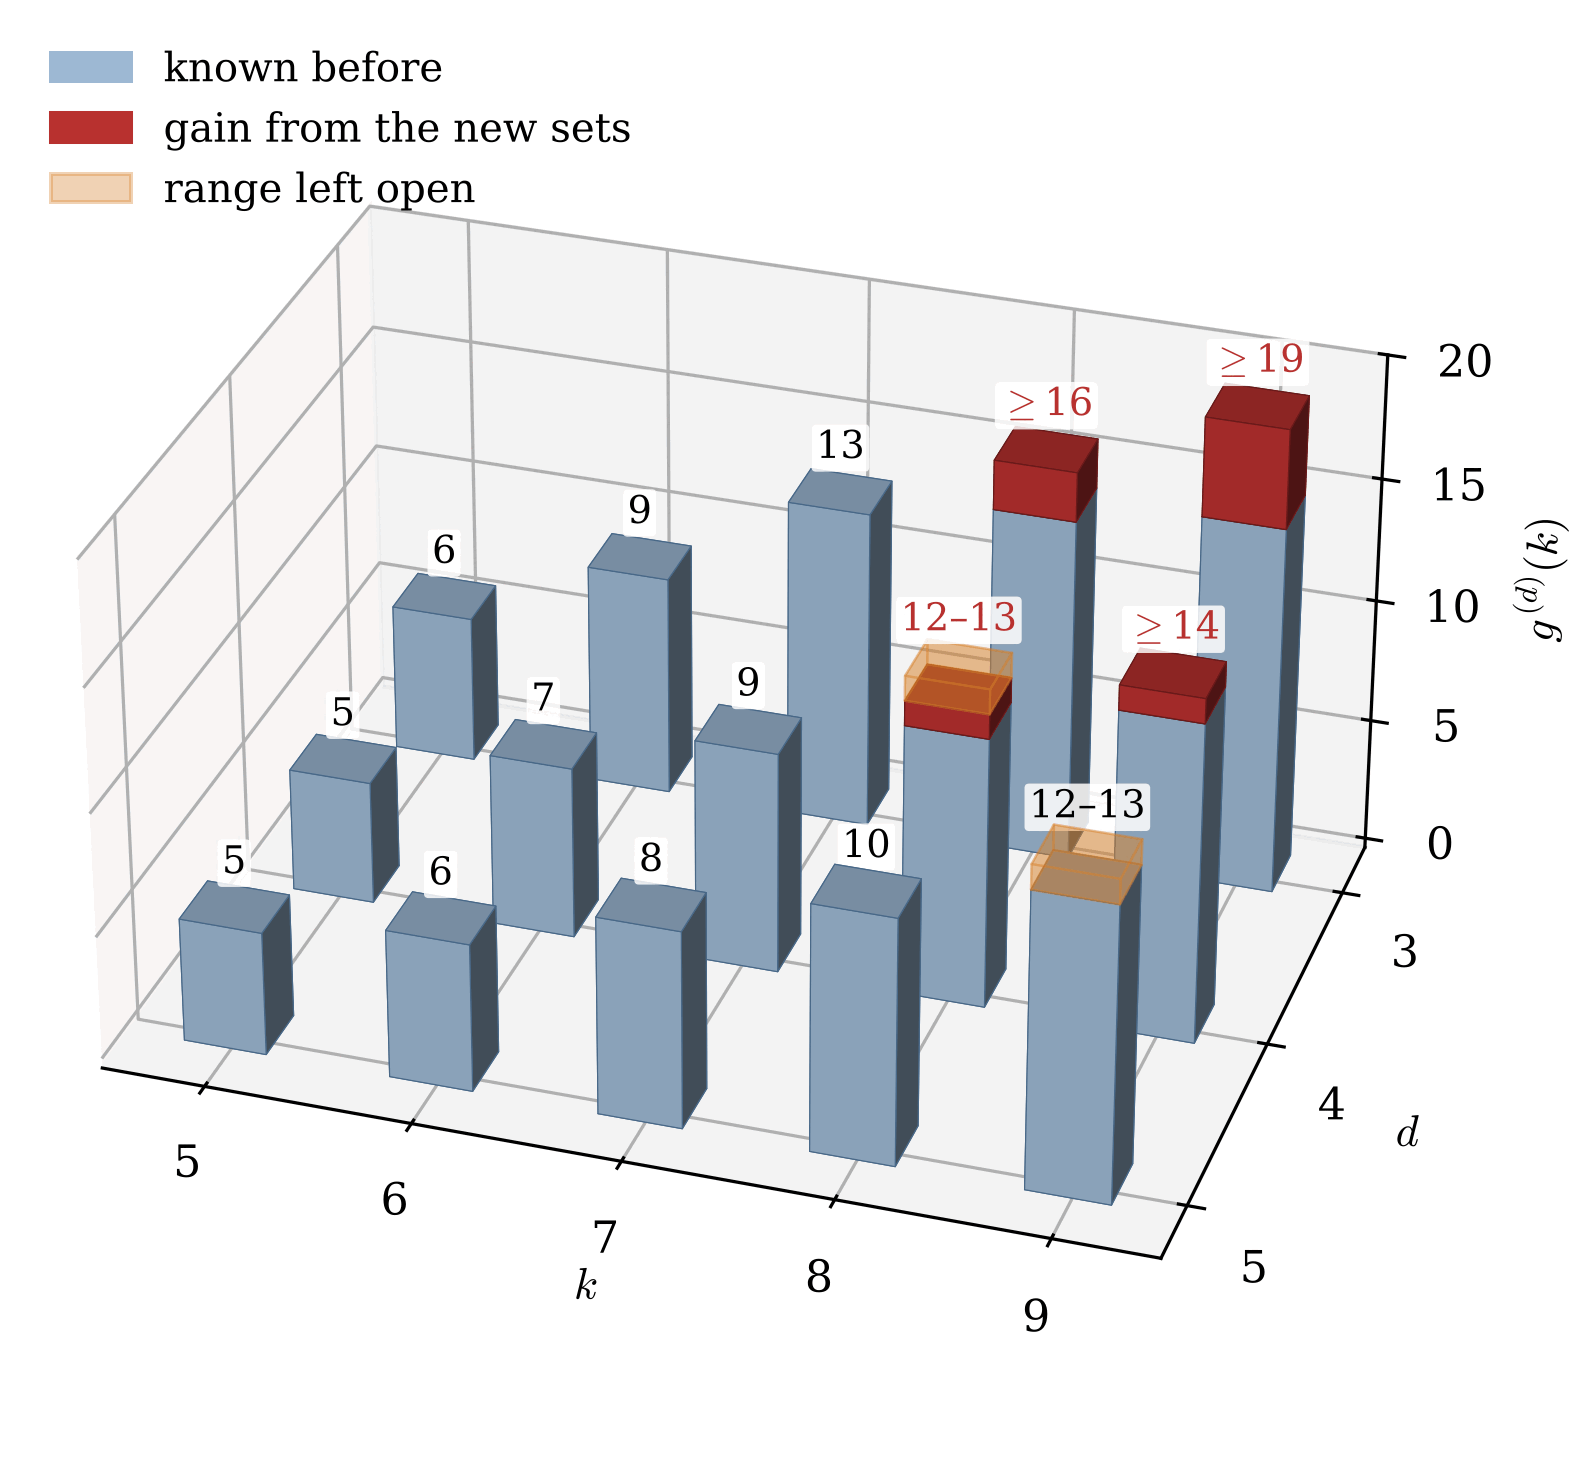
\includegraphics[width=\columnwidth]{figures/fig_bounds.png}
\caption{The values of $g^{(d)}(k)$ for $d=3,4,5$ and $k=5,\dots,9$. Blue bars are the values or lower bounds known before; red bars show the gain from Theorems~\ref{thm:A}, \ref{thm:B} and~\ref{thm:C}; the light orange blocks mark the ranges left open below Scheucher's upper bounds. Where no upper bound is drawn, only the lower bound is shown.}\label{fig:bounds}
\end{figure}

We prove the following three theorems.

\begin{mainthm}\label{thm:A}
There is a set of eleven points in general position in $\R^4$ with no eight points in convex position. Consequently $g^{(4)}(8)\ge12$ and $h^{(4)}(8)\ge12$, and by \eqref{eq:scheucher} both numbers lie in $\{12,13\}$.
\end{mainthm}

\begin{mainthm}\label{thm:B}
There is a set of fifteen points in general position in $\R^3$ with no eight points in convex position. Consequently $g^{(3)}(8)\ge16$ and $h^{(3)}(8)\ge16$.
\end{mainthm}

\begin{mainthm}\label{thm:C}
There is a set of thirteen points in general position in $\R^4$ with no nine points in convex position, and a set of eighteen points in general position in $\R^3$ with no nine points in convex position. Consequently $g^{(4)}(9)\ge14$, $h^{(4)}(9)\ge14$, $g^{(3)}(9)\ge19$, $h^{(3)}(9)\ge19$ and $g^{(3)}(10)\ge20$.
\end{mainthm}

Theorem~\ref{thm:A} is the first lower bound beyond \eqref{eq:linear} in four dimensions, and it leaves two candidates for $g^{(4)}(8)$; the conjecture of Morris and Soltan and Scheucher's conjecture both predict $13$. Theorem~\ref{thm:B} raises the lower bound for $g^{(3)}(8)$ by two; the conjecture of Morris and Soltan predicts $g^{(3)}(8)=4g^{(3)}(5)-3=21$, and the best upper bound we know comes from dimension reduction and the planar estimate of T\'oth and Valtr, as in \cite{Sch23}. Theorem~\ref{thm:C} raises the lower bound for $g^{(4)}(9)$ from the value $2k-d-1=13$ of the construction of Bisztriczky and Harborth to $14$, and the lower bound for $g^{(3)}(9)$ from $g^{(3)}(7)+2=15$ to $19$; the conjecture of Morris and Soltan predicts $g^{(4)}(9)=4g^{(4)}(5)-3=17$ and $g^{(3)}(9)=4g^{(3)}(6)-3=33$.\footnote{For $g^{(3)}(10)$ the construction of Bisztriczky and Harborth gives $16$, and Theorem~\ref{thm:C} with the monotonicity of the previous footnote gives $20$. In $\R^4$ the bound $g^{(4)}(10)\ge g^{(4)}(9)+1=15$ coincides with $2k-d-1=15$, so Theorem~\ref{thm:C} gives nothing new there.}

All the proofs are certificates. If $v_0,\dots,v_d$ are affinely independent points of $\R^d$ and
\begin{equation}\label{eq:relation}
\sum_{j=0}^{d} m_j v_j=M p,\qquad m_j\in\{1,2,3,\dots\},\quad M=\sum_{j=0}^d m_j,
\end{equation}
then $p$ lies in the interior of the simplex spanned by the $v_j$, and no set containing $p$ and the $v_j$ is in convex position. We call \eqref{eq:relation} a \emph{relation}. A set has no $k$-gon as soon as every $k$ of its points contain the $d+2$ points of some relation (Proposition~\ref{prop:cover}). Twenty-eight relations prove Theorem~\ref{thm:A}, $\relB$ prove Theorem~\ref{thm:B}, and $\relCfour$ and $\relCthree$ prove the two parts of Theorem~\ref{thm:C}; they are listed in Appendix~\ref{app:certA}. Each relation is an identity between integer vectors that can be checked by hand. That the relations meet every $8$-subset is a finite combinatorial condition: for Theorem~\ref{thm:A} it is a statement about $165$ triples, which Table~\ref{tab:certA} lets the reader check directly, and for Theorem~\ref{thm:B} it concerns $6435$ subsets and is checked by the programs of the archive. For the thirteen points of Theorem~\ref{thm:C} it concerns the $715$ four-element complements of $9$-subsets, again listed through Table~\ref{tab:certCfour}, and for the eighteen points the $48620$ subsets of size nine. Since relations survive small perturbations (Lemma~\ref{lem:stable}), general position costs nothing; the integer sets we give are in general position as they stand.

The two sets have a layered structure (Figures~\ref{fig:fourd} and~\ref{fig:layers}). The eleven points in $\R^4$ consist of the six vertices of a bipyramid over a tetrahedron and five points inside it, and every relation places one of the five inner points in a simplex. The fifteen points in $\R^3$ form three convex layers, a triangular bipyramid, an octahedron and a tetrahedron, and no relation places a vertex of the outer bipyramid inside a simplex. Scheucher's twelve points in $\R^3$ without a $7$-gon have convex layers of sizes $5$, $6$ and $1$, again a triangular bipyramid and an octahedron. The sets of Theorem~\ref{thm:C} are built the same way (Figures~\ref{fig:ninefour} and~\ref{fig:ninethree}). The thirteen points in $\R^4$ are the seven vertices of a $4$-simplex with two caps and six points inside it forming a cyclic polytope. The eighteen points in $\R^3$ form a capped octahedron, a pentagonal bipyramid and a tetrahedron, and again only points of the two inner layers lie inside simplices. For other extremal problems on explicit configurations in dimensions four and seven see \cite{BBB26a,BBB26b}, and for reflexive polytopes in dimension four see \cite{Bha26}.

Section~\ref{sec:cert} proves the certificate criterion, Sections~\ref{sec:A}, \ref{sec:B} and~\ref{sec:C} prove Theorems~\ref{thm:A}, \ref{thm:B} and~\ref{thm:C}, Section~\ref{sec:search} explains how the sets were found, and Section~\ref{sec:open} discusses what remains open. Appendix~\ref{app:proofs} contains the detailed proofs of the lemmas of Section~\ref{sec:cert}, and Appendix~\ref{app:certA} the four certificates.

%----------------------------------------------------------------------
\section{Relations and certificates}\label{sec:cert}

Throughout, $X$ is a finite set in $\R^d$ and $\conv$, $\inter$ denote the convex hull and the interior. For points $v_0,\dots,v_d$ write $\det(v_0,\dots,v_d)$ for the determinant of the $(d+1)\times(d+1)$ matrix whose rows are $(1,v_j)$; it vanishes exactly when the points lie on a common hyperplane, and its absolute value is $d!$ times the volume of the simplex they span.

\begin{lemma}\label{lem:caratheodory}
Let $X$ be in general position and $Y\subseteq X$. Then $Y$ is in convex position if and only if no point of $Y$ lies in $\inter\conv\sigma$ for a set $\sigma$ of $d+1$ other points of $Y$.
\end{lemma}

\begin{proof}
If $p\in\inter\conv\sigma$ with $\sigma\subseteq Y\setminus\{p\}$, then $p\in\conv(Y\setminus\{p\})$ and $Y$ is not in convex position. Conversely, suppose $p\in\conv(Y\setminus\{p\})$. By Carath\'eodory's theorem \cite{Gru03} $p$ is a convex combination of affinely independent points $v_0,\dots,v_r$ of $Y\setminus\{p\}$, and we choose $r$ minimal, so all coefficients are positive. If $r<d$, then $p$ and $v_0,\dots,v_r$ are $r+2\le d+1$ points on an $r$-dimensional affine subspace, hence on a hyperplane, contrary to general position. So $r=d$, the simplex $\conv\{v_0,\dots,v_d\}$ is full-dimensional, and a point with positive barycentric coordinates lies in its interior.
\end{proof}

\begin{definition}\label{def:relation}
A \emph{relation} of $X$ is a triple $(p,\sigma,m)$ where $p\in X$, $\sigma=\{v_0,\dots,v_d\}\subseteq X\setminus\{p\}$ satisfies $\det(v_0,\dots,v_d)\ne0$, and $m=(m_0,\dots,m_d)$ consists of positive integers with $\sum_jm_jv_j=Mp$, $M=\sum_jm_j$. Its \emph{support} is $\{p\}\cup\sigma$, a set of $d+2$ points.
\end{definition}

\begin{figure}[tb]
\centering
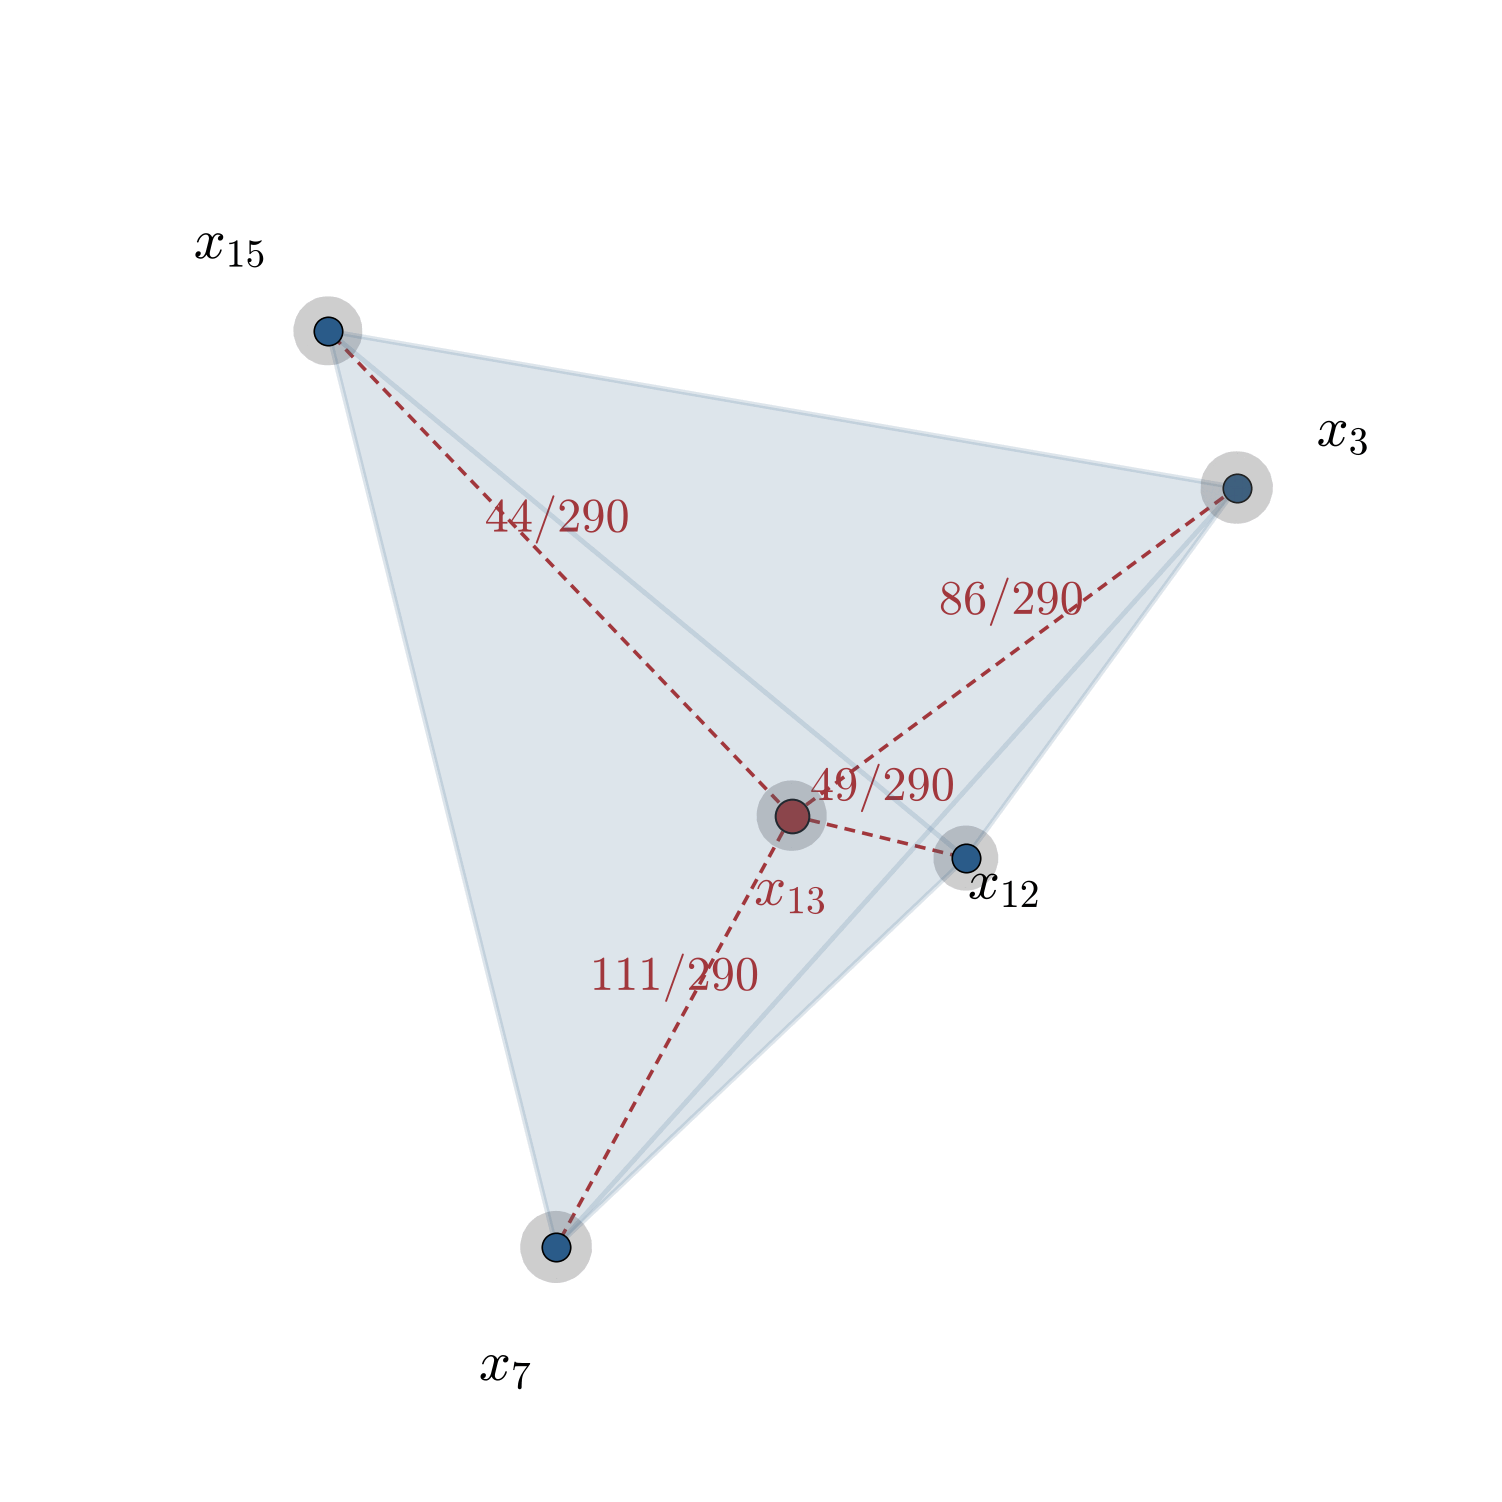
\includegraphics[width=\columnwidth]{figures/fig_relation.png}
\caption{One relation of the set of Theorem~\ref{thm:B}, drawn after an affine map that turns the simplex into a regular tetrahedron and keeps barycentric coordinates. The point $p$ is the weighted mean of the four vertices with the positive integer weights shown. The small balls indicate that every point may move a little without $p$ leaving the simplex (Lemma~\ref{lem:stable}).}\label{fig:relation}
\end{figure}

\begin{lemma}\label{lem:interior}
If $(p,\sigma,m)$ is a relation, then $p\in\inter\conv\sigma$, the barycentric coordinates of $p$ with respect to $\sigma$ are $m_j/M$, and if the points have integer coordinates and $\gcd(m_0,\dots,m_d)=1$, then $M$ divides $\det(v_0,\dots,v_d)$.
\end{lemma}

\begin{proof}
The $v_j$ are affinely independent, so every point has unique barycentric coordinates with respect to them, and \eqref{eq:relation} shows that those of $p$ are $m_j/M>0$. Write $D=\det(v_0,\dots,v_d)$ and let $N_j$ be the same determinant with $v_j$ replaced by $p$. By Cramer's rule the $j$th barycentric coordinate of $p$ is $N_j/D$ (Appendix~\ref{app:proofs}), so $m_jD=MN_j$ for every $j$. The right-hand sides are integer multiples of $M$, and an integer combination of the $m_j$ equals $1$, hence $M$ divides $\det(v_0,\dots,v_d)$.
\end{proof}

In the tables of the appendices we record, for each relation, the integer $g=|\det(v_0,\dots,v_d)|/M$. A reader who checks one determinant per relation thereby also checks $\det\ne0$; Lemma~\ref{lem:interior} explains why $g$ is always an integer.

\begin{lemma}\label{lem:stable}
Let $(p,\sigma,m)$ be a relation of $X$. There is $\varepsilon>0$ such that for every map $x\mapsto x'$ with $|x'-x|<\varepsilon$ on the support, $p'$ lies in the interior of the simplex spanned by the images of $\sigma$.
\end{lemma}

\begin{proof}
The barycentric coordinates of $p$ with respect to $\sigma$ are rational functions of the coordinates of the $d+2$ points whose common denominator is $\det(v_0,\dots,v_d)$. They are therefore continuous where this determinant does not vanish, and at the given points they are positive. Continuity gives an $\varepsilon$ that keeps the determinant nonzero and the coordinates positive. Appendix~\ref{app:proofs} gives an explicit $\varepsilon$.
\end{proof}

\begin{proposition}\label{prop:cover}
Let $X$ be a finite set in $\R^d$ and $\mathcal{R}$ a set of relations of $X$ such that every $k$-subset of $X$ contains the support of some relation in $\mathcal{R}$. Then $X$ contains no $k$ points in convex position. Moreover, there is a set $X'$ in general position, obtained from $X$ by moving each point by an arbitrarily small amount, with the same property.
\end{proposition}

\begin{proof}
Let $Y\subseteq X$ have $k$ points and let $(p,\sigma,m)$ be a relation with support in $Y$. By Lemma~\ref{lem:interior}, $p\in\conv\sigma\subseteq\conv(Y\setminus\{p\})$, so $Y$ is not in convex position. For the second statement let $\varepsilon$ be the least of the constants of Lemma~\ref{lem:stable} over the finitely many relations of $\mathcal R$. The configurations of $|X|$ points in $\R^d$ that are not in general position form the zero set of the product of the polynomials $\det(x_{i_0},\dots,x_{i_d})$, none of which vanishes identically, so they form a closed set with empty interior in $\R^{d|X|}$. Hence there are points $x'$ with $|x'-x|<\varepsilon$ in general position. Every relation of $\mathcal R$ still places $p'$ in the interior of the image simplex, so the first argument applies to $X'$.
\end{proof}

The condition of Proposition~\ref{prop:cover} can be stated through complements. A $k$-subset $Y$ contains the support $S$ of a relation if and only if $X\setminus Y\subseteq X\setminus S$. So if $|X|=n$, the sets $X\setminus S$ of size $n-d-2$ must cover every $(n-k)$-subset of $X$. This is a covering design, and Sch\"onheim's bound \cite{Sch64} gives a lower bound for the number of relations any such certificate needs.

\begin{remark}\label{rem:schoenheim}
A certificate in the sense of Proposition~\ref{prop:cover} for eleven points in $\R^4$ and $k=8$ covers the $3$-subsets of an $11$-set by $5$-sets, and needs at least $\lceil\frac{11}{5}\lceil\frac{10}{4}\lceil\frac{9}{3}\rceil\rceil\rceil=18$ relations. For fifteen points in $\R^3$ and $k=8$ it covers the $7$-subsets of a $15$-set by $10$-sets, and needs at least $74$ relations. For $k=9$ the thirteen points in $\R^4$ need at least $26$ relations and the eighteen points in $\R^3$ at least $85$. Our certificates use $\relA$, $\relB$, $\relCfour$ and $\relCthree$ relations.
\end{remark}

By Lemma~\ref{lem:caratheodory} the method is complete: if a set in general position has no $k$-gon, then every $k$-subset contains a point in the interior of a simplex of other points of the subset, and when the coordinates are rational the barycentric coordinates are rational, so the relation can be written with integer weights. A certificate exists exactly when the set has no $k$-gon.

%----------------------------------------------------------------------
\section{Eleven points in four-space}\label{sec:A}

Let $X_4=\{x_1,\dots,x_{11}\}\subset\R^4$ be the points of Table~\ref{tab:coordsA}. All coordinates lie between $0$ and $\maxcoordA$.

\begin{table}[tb]
\caption{The eleven points of Theorem~\ref{thm:A} in $\mathbb{R}^4$.}\label{tab:coordsA}
\begin{ruledtabular}
\begin{tabular}{rrrrr}
point & $x$ & $y$ & $z$ & $w$ \\ \hline
$x_{1}$ & 0 & 19 & 34 & 30 \\
$x_{2}$ & 2 & 36 & 25 & 0 \\
$x_{3}$ & 18 & 0 & 19 & 1 \\
$x_{4}$ & 19 & 18 & 40 & 32 \\
$x_{5}$ & 20 & 32 & 0 & 23 \\
$x_{6}$ & 23 & 31 & 15 & 1 \\
$x_{7}$ & 12 & 16 & 24 & 14 \\
$x_{8}$ & 13 & 27 & 21 & 13 \\
$x_{9}$ & 16 & 24 & 14 & 17 \\
$x_{10}$ & 16 & 25 & 19 & 25 \\
$x_{11}$ & 18 & 24 & 20 & 14 \\
\end{tabular}
\end{ruledtabular}
\end{table}


\begin{proposition}\label{prop:structureA}
The convex hull of $X_4$ is a bipyramid over a tetrahedron: its vertices are $x_1,\dots,x_6$, and its eight facets are the tetrahedra spanned by $x_1$ or $x_6$ together with three of $x_2,x_3,x_4,x_5$. The points $x_7,\dots,x_{11}$ lie in the interior.
\end{proposition}

\begin{proof}
For each of the eight listed quadruples $\tau$ the determinants $\det(\tau,x)$ have one sign for all seven remaining points $x$ of $X_4$, which is a sign check of $56$ determinants. So the hyperplane through $\tau$ supports $\conv X_4$, and since $\tau$ consists of four affinely independent points it spans a facet. Each triangle contained in one of these eight tetrahedra lies in exactly two of them. In a convex polytope every ridge lies in exactly two facets and the facets are connected through ridges \cite{Zie95}, so these eight tetrahedra are all the facets of $\conv X_4$, and they are the facets of the bipyramid $\conv\{x_1,\dots,x_6\}$. The points $x_7,\dots,x_{11}$ lie strictly on the inner side of all eight facet hyperplanes, by the same sign check, so they are interior.
\end{proof}

\begin{figure*}[tp]
\centering
\begin{minipage}[t]{0.485\textwidth}\centering
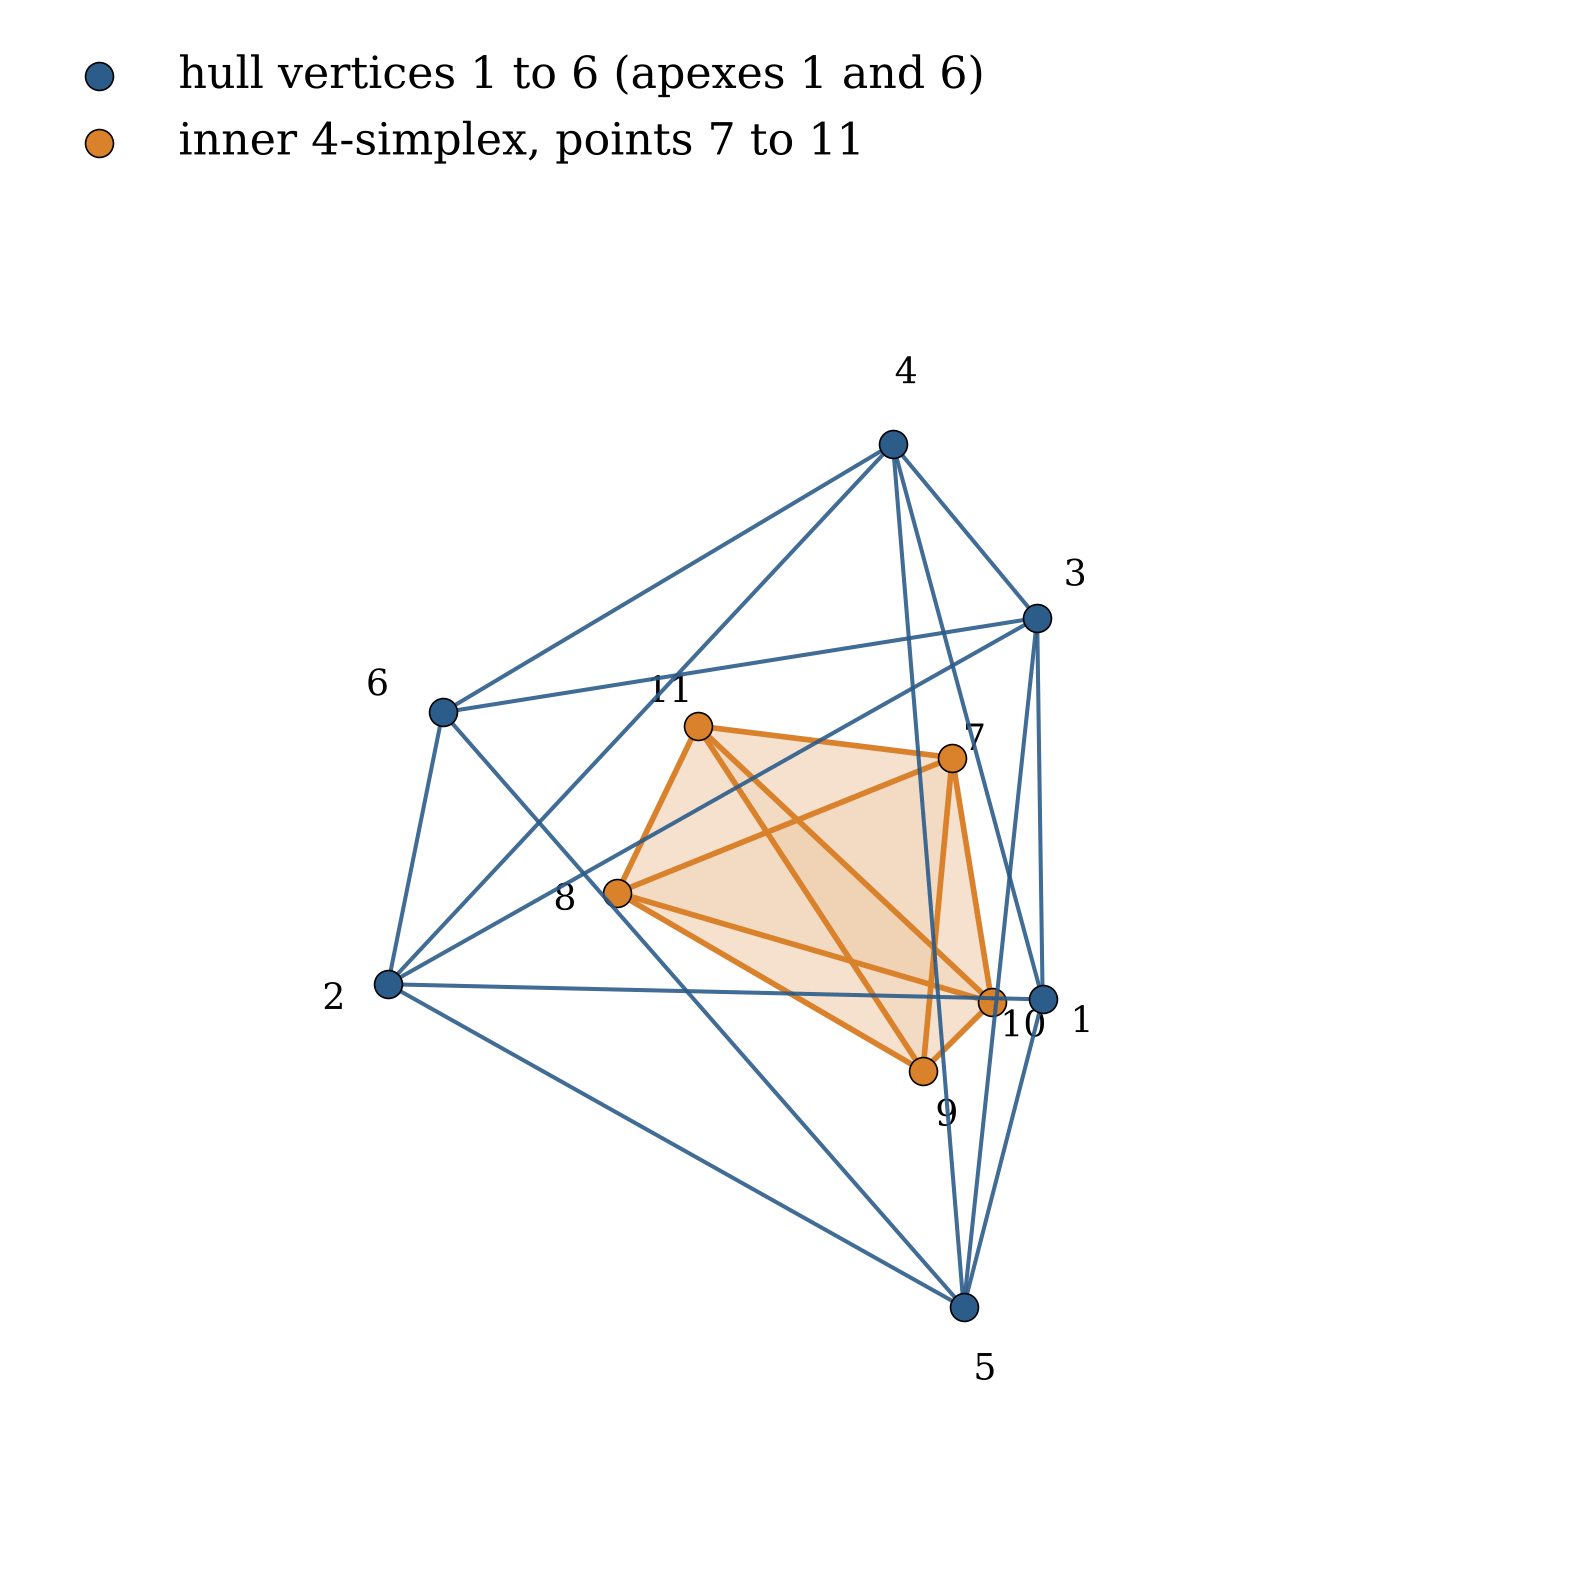
\includegraphics[width=\linewidth]{figures/fig_fourd.png}
\caption{A schematic view of the set of Theorem~\ref{thm:A}, projected to three dimensions after an affine map that makes the hull a regular bipyramid. The tetrahedron $x_2x_3x_4x_5$ and the apexes $x_1$, $x_6$ span the hull; the five inner points (red) form a $4$-simplex, drawn enlarged. Every one of the $\relA$ relations of Table~\ref{tab:certA} places a red point inside a simplex of other points.}\label{fig:fourd}
\end{minipage}\hfill
\begin{minipage}[t]{0.485\textwidth}\centering
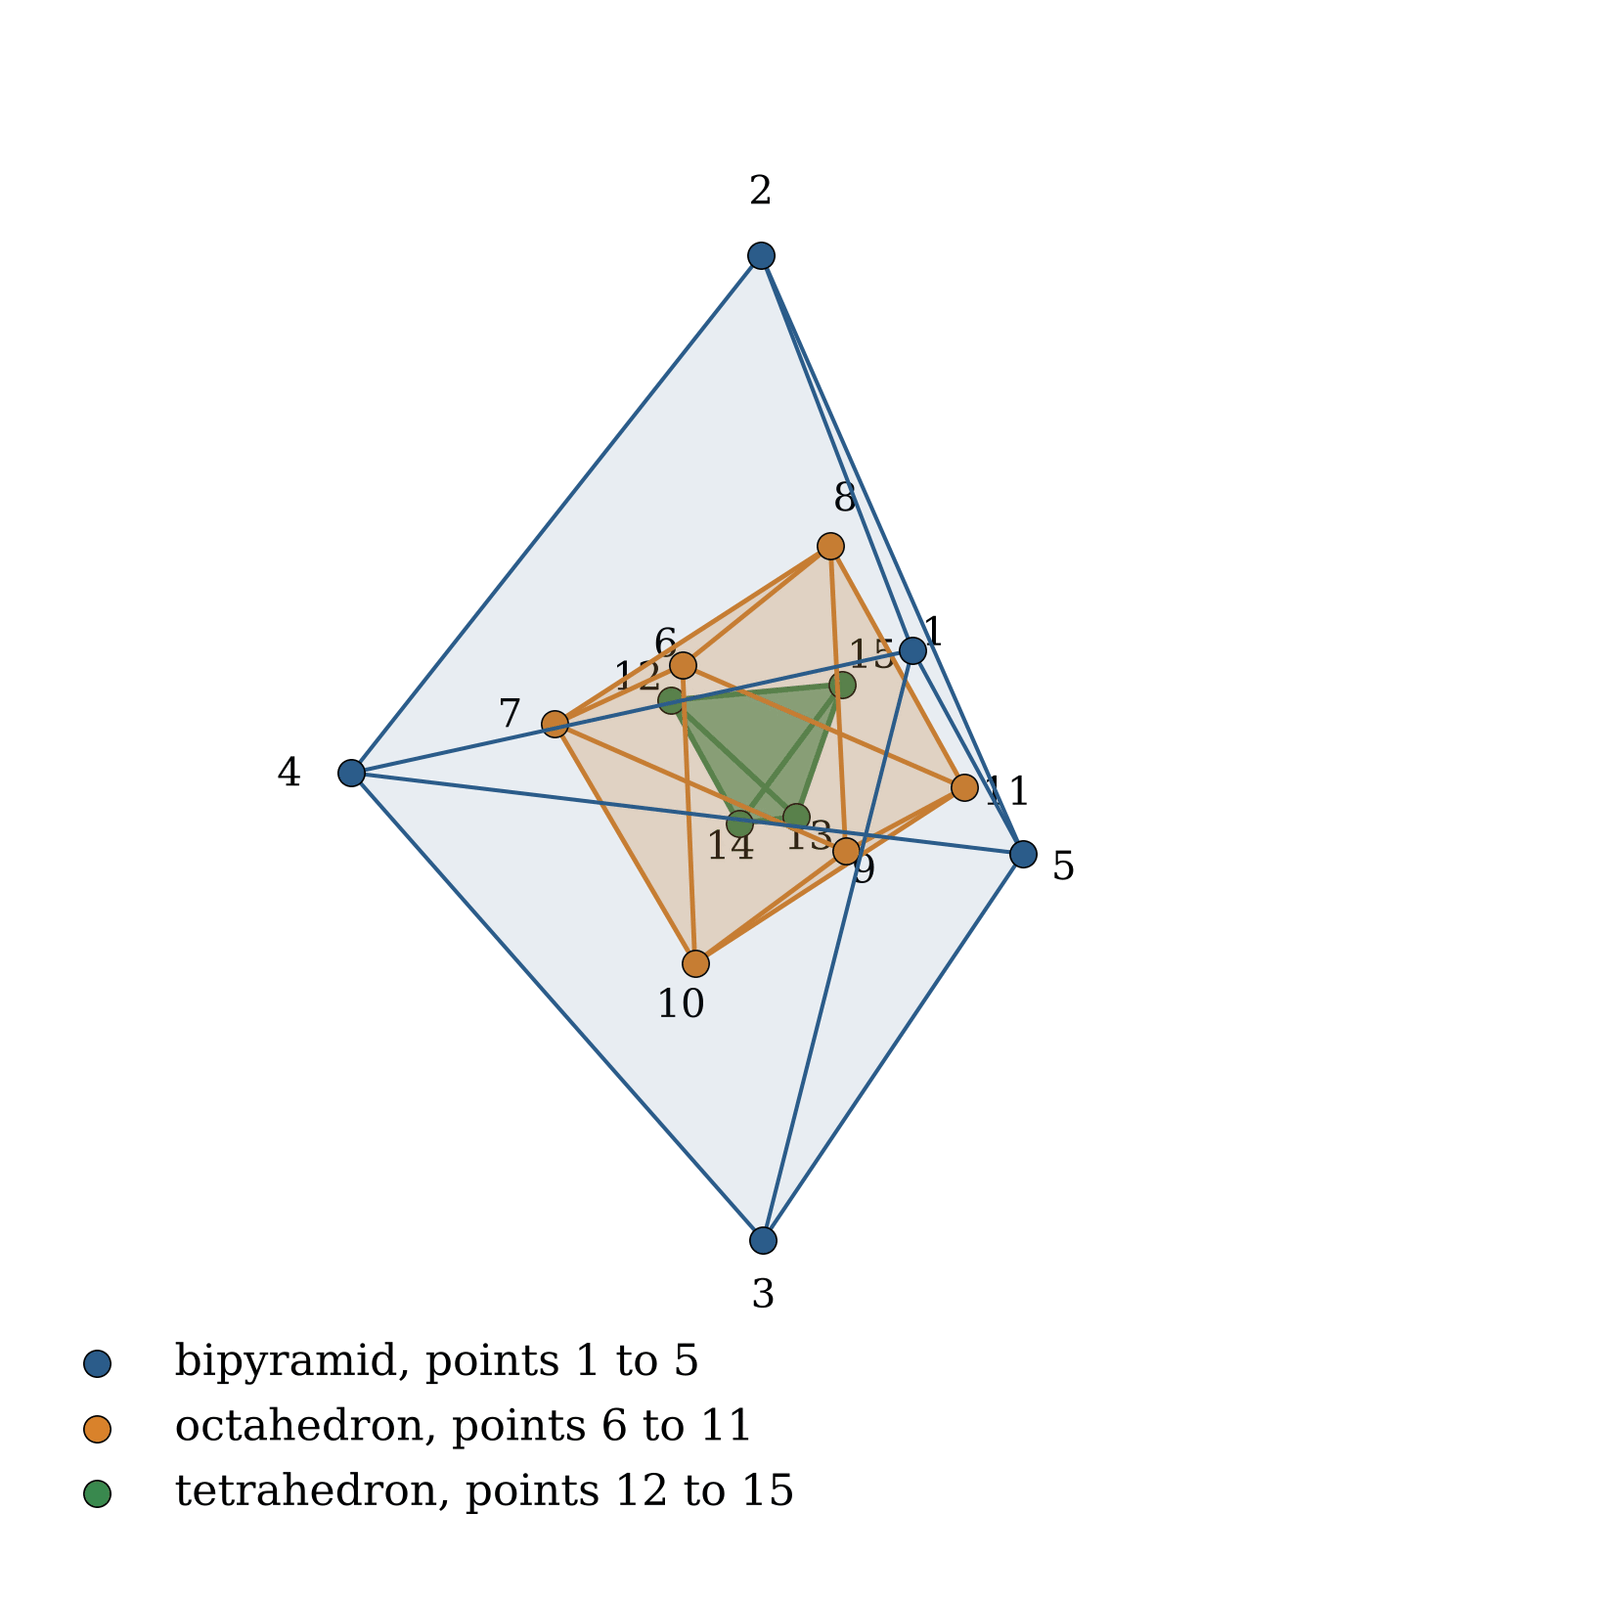
\includegraphics[width=\linewidth]{figures/fig_layers.png}
\caption{The three convex layers of the set of Theorem~\ref{thm:B}: a triangular bipyramid (blue), an octahedron (green) and a tetrahedron (red), with the labels of Table~\ref{tab:coordsB}. The drawing is schematic: it shows regular solids with the true combinatorics and labels, since in the actual coordinates the inner layers are small and flat.}\label{fig:layers}
\end{minipage}
\end{figure*}

\begin{proof}[Proof of Theorem~\ref{thm:A}]
Each row of Table~\ref{tab:certA} is a relation of $X_4$: the identity $\sum_jm_jx_{s_j}=Mx_p$ holds in each of the four coordinates, the weights are positive, and the determinant of the simplex is $\pm gM\ne0$. The last column of the table lists, for each relation, the five points outside its support. Every one of the $\binom{11}{3}=165$ triples of indices lies in one of these $\relA$ five-element sets. So the complement of every $8$-subset of $X_4$ lies outside the support of some relation, that is, every $8$-subset contains a support, and Proposition~\ref{prop:cover} shows that $X_4$ has no $8$ points in convex position. The set $X_4$ is itself in general position: the $\binom{11}{5}=462$ determinants of five of its points are all nonzero, the smallest in absolute value being $\mindetA$. Independently of this check, Proposition~\ref{prop:cover} provides a perturbation of $X_4$ in general position with the same property. Hence $g^{(4)}(8)\ge12$. An $8$-hole is an $8$-gon, so $h^{(4)}(8)\ge g^{(4)}(8)\ge12$, and Scheucher's bound $h^{(4)}(8)\le13$ \cite{Sch23} together with $g^{(4)}(8)\le h^{(4)}(8)$ gives the last statement.
\end{proof}

Every relation places one of the inner points $x_7,\dots,x_{11}$ in a simplex; the outer points are vertices of the hull and lie inside nothing. Any eight points of $X_4$ include at least two inner points, and the certificate shows that one of the inner points among them always lies inside a simplex spanned by four or five of the others.

%----------------------------------------------------------------------
\section{Fifteen points in three-space}\label{sec:B}

Let $X_3=\{x_1,\dots,x_{15}\}\subset\R^3$ be the points of Table~\ref{tab:coordsB}. All coordinates lie between $0$ and $\maxcoordB$.

\begin{table}[tb]
\caption{The fifteen points of Theorem~\ref{thm:B} in $\mathbb{R}^3$.}\label{tab:coordsB}
\begin{ruledtabular}
\begin{tabular}{rrrr}
point & $x$ & $y$ & $z$ \\ \hline
$x_{1}$ & 0 & 128 & 0 \\
$x_{2}$ & 53 & 0 & 130 \\
$x_{3}$ & 92 & 166 & 46 \\
$x_{4}$ & 110 & 180 & 108 \\
$x_{5}$ & 171 & 139 & 79 \\
$x_{6}$ & 73 & 88 & 95 \\
$x_{7}$ & 75 & 161 & 71 \\
$x_{8}$ & 79 & 143 & 55 \\
$x_{9}$ & 98 & 169 & 67 \\
$x_{10}$ & 110 & 176 & 104 \\
$x_{11}$ & 123 & 128 & 82 \\
$x_{12}$ & 81 & 109 & 93 \\
$x_{13}$ & 85 & 154 & 67 \\
$x_{14}$ & 86 & 154 & 66 \\
$x_{15}$ & 101 & 163 & 69 \\
\end{tabular}
\end{ruledtabular}
\end{table}


\begin{proposition}\label{prop:structureB}
The set $X_3$ has three convex layers. The vertices of $\conv X_3$ are $x_1,\dots,x_5$, forming a triangular bipyramid with apexes \LAYERONEAPEX{} over the triangle \LAYERONEBASE. The vertices of the convex hull of the remaining points are $x_6,\dots,x_{11}$, forming an octahedron whose opposite vertices are \LAYERTWOPAIRS. The points $x_{12},\dots,x_{15}$ span a tetrahedron inside it.
\end{proposition}

\begin{proof}
As for Proposition~\ref{prop:structureA}. The six triangles of the bipyramid have constant sign of $\det(\tau,x)$ over the other twelve points of $X_3$, so they are facets of $\conv X_3$; every edge among them lies in exactly two, so they are all the facets, and the remaining ten points lie strictly inside. The eight triangles of the octahedron have constant sign over the other seven points of $\{x_6,\dots,x_{15}\}$ and close up in the same way, so they are the facets of the second layer, with $x_{12},\dots,x_{15}$ strictly inside. Four points in general position span a tetrahedron.
\end{proof}

\begin{proof}[Proof of Theorem~\ref{thm:B}]
Each row of Tables~\ref{tab:certB} and~\ref{tab:certBb} is a relation of $X_3$, by the same three checks as before. Every one of the $\binom{15}{8}=6435$ eight-point subsets of $X_3$ contains the support of one of these $\relB$ relations; equivalently, every $7$-subset of the indices lies in the complement of a support. This finite statement is verified in the archive \cite{BB26z} by independent programs in four languages and by the Lean~4 kernel; three of the programs also test every $8$-subset directly for convex position in exact integer arithmetic, without using the certificate. Proposition~\ref{prop:cover} then shows that $X_3$ has no $8$ points in convex position. The set $X_3$ is in general position, the smallest absolute value of its $\binom{15}{4}=1365$ determinants being $\mindetB$, and again Proposition~\ref{prop:cover} would supply a perturbation if this check were omitted. So $g^{(3)}(8)\ge16$ and $h^{(3)}(8)\ge16$, and the monotonicity $g^{(3)}(9)\ge g^{(3)}(8)+1$ gives $g^{(3)}(9)\ge17$.
\end{proof}

The points $p$ of the relations run through all ten points of the two inner layers, and no relation places a vertex of the outer bipyramid inside a simplex. In $\relBinner$ of the $\relB$ relations the point $p$ is a vertex of the inner tetrahedron. The others are needed because an $8$-subset may avoid the inner tetrahedron altogether: it then consists of eight of the eleven points of the two outer layers, and one of its octahedron vertices must lie inside a simplex of the others.

%----------------------------------------------------------------------
\section{Nine points}\label{sec:C}

Let $Y_4=\{x_1,\dots,x_{13}\}\subset\R^4$ be the points of Table~\ref{tab:coordsCfour} and $Y_3=\{x_1,\dots,x_{18}\}\subset\R^3$ those of Table~\ref{tab:coordsCthree}; within this section the labels $x_i$ refer to these two tables. All coordinates lie between $0$ and $\maxcoordCfour$ in $\R^4$ and between $0$ and $\maxcoordCthree$ in $\R^3$.

\begin{table}[tb]
\caption{The thirteen points of Theorem~\ref{thm:C} in $\mathbb{R}^4$.}\label{tab:coordsCfour}
\begin{ruledtabular}
\begin{tabular}{rrrrr}
point & $x$ & $y$ & $z$ & $w$ \\ \hline
$x_{1}$ & 0 & 2 & 46 & 23 \\
$x_{2}$ & 2 & 19 & 7 & 50 \\
$x_{3}$ & 10 & 0 & 0 & 0 \\
$x_{4}$ & 27 & 20 & 42 & 23 \\
$x_{5}$ & 36 & 1 & 26 & 30 \\
$x_{6}$ & 39 & 21 & 23 & 15 \\
$x_{7}$ & 47 & 11 & 21 & 26 \\
$x_{8}$ & 12 & 9 & 8 & 23 \\
$x_{9}$ & 26 & 12 & 19 & 29 \\
$x_{10}$ & 27 & 10 & 26 & 22 \\
$x_{11}$ & 30 & 9 & 25 & 25 \\
$x_{12}$ & 30 & 11 & 20 & 18 \\
$x_{13}$ & 30 & 16 & 26 & 21 \\
\end{tabular}
\end{ruledtabular}
\end{table}

\begin{table}[tb]
\caption{The eighteen points of Theorem~\ref{thm:C} in $\mathbb{R}^3$.}\label{tab:coordsCthree}
\begin{ruledtabular}
\begin{tabular}{rrrr}
point & $x$ & $y$ & $z$ \\ \hline
$x_{1}$ & 0 & 150 & 13 \\
$x_{2}$ & 15 & 90 & 8 \\
$x_{3}$ & 17 & 88 & 133 \\
$x_{4}$ & 60 & 0 & 67 \\
$x_{5}$ & 93 & 39 & 2 \\
$x_{6}$ & 96 & 50 & 80 \\
$x_{7}$ & 107 & 143 & 0 \\
$x_{8}$ & 45 & 82 & 28 \\
$x_{9}$ & 50 & 92 & 25 \\
$x_{10}$ & 59 & 47 & 60 \\
$x_{11}$ & 60 & 36 & 56 \\
$x_{12}$ & 69 & 59 & 18 \\
$x_{13}$ & 77 & 53 & 17 \\
$x_{14}$ & 79 & 59 & 56 \\
$x_{15}$ & 59 & 67 & 33 \\
$x_{16}$ & 62 & 64 & 32 \\
$x_{17}$ & 70 & 62 & 26 \\
$x_{18}$ & 73 & 64 & 50 \\
\end{tabular}
\end{ruledtabular}
\end{table}


\begin{proposition}\label{prop:structureCfour}
The vertices of $\conv Y_4$ are $x_1,\dots,x_7$, and its thirteen facets are $x_2x_3x_4x_6$, the six tetrahedra $x_1\tau$ with $\tau$ one of the triangles $x_2x_3x_4$, $x_2x_3x_5$, $x_2x_4x_5$, $x_3x_4x_6$, $x_3x_5x_6$, $x_4x_5x_6$, and the six tetrahedra $x_7\tau$ with $\tau$ one of $x_2x_3x_5$, $x_2x_3x_6$, $x_2x_4x_5$, $x_2x_4x_6$, $x_3x_5x_6$, $x_4x_5x_6$. So $\conv Y_4$ arises from the $4$-simplex $\conv\{x_2,\dots,x_6\}$ by placing $x_1$ beyond its facets $x_2x_3x_4x_5$ and $x_3x_4x_5x_6$ and then $x_7$ beyond its facets $x_2x_3x_5x_6$ and $x_2x_4x_5x_6$, and every two vertices except $x_1,x_7$ span an edge. The points $x_8,\dots,x_{13}$ lie in the interior and are the vertices of a polytope combinatorially equivalent to the cyclic polytope $C_4(6)$.
\end{proposition}

\begin{proof}
The sign check of Proposition~\ref{prop:structureA} applies to the thirteen listed tetrahedra: for each of them the determinants $\det(\tau,x)$ have one sign over the other nine points of $Y_4$, and the remaining six points lie strictly on the inner side of all thirteen hyperplanes. Every triangle of one of the thirteen tetrahedra lies in exactly two of them, so they are all the facets. Placing a point beyond a set of facets of a polytope, and beneath the others, replaces the visible facets by the cones from the point over the boundary of their union \cite[Theorem~5.2.1]{Gru03}; the two visible facets of $\conv\{x_2,\dots,x_6\}$ for $x_1$ share the triangle $x_3x_4x_5$, the two for $x_7$ share $x_2x_5x_6$, and the facets listed are exactly those this rule produces. The convex hull of $x_8,\dots,x_{13}$ has nine facets,
\[
\begin{gathered}
x_8x_9x_{10}x_{11},\ x_8x_9x_{10}x_{13},\ x_8x_9x_{11}x_{12},\ x_8x_9x_{12}x_{13},\ x_8x_{10}x_{11}x_{12},\\
x_8x_{10}x_{12}x_{13},\ x_9x_{10}x_{11}x_{13},\ x_9x_{11}x_{12}x_{13},\ x_{10}x_{11}x_{12}x_{13},
\end{gathered}
\]
by the same check, and every two of its six vertices span an edge. A neighbourly simplicial $4$-polytope with six vertices is combinatorially the cyclic polytope \cite{Gru03}.
\end{proof}

\begin{proposition}\label{prop:structureCthree}
The set $Y_3$ has three convex layers. The first, with vertices $x_1,\dots,x_7$, is the octahedron with vertices $x_2,\dots,x_7$ and opposite pairs $\{x_2,x_6\}$, $\{x_3,x_5\}$, $\{x_4,x_7\}$, capped by $x_1$ over its face $x_2x_3x_7$. The second, with vertices $x_8,\dots,x_{14}$, is a pentagonal bipyramid with apexes $x_9$ and $x_{11}$ over the pentagon $x_8x_{10}x_{14}x_{13}x_{12}$. The points $x_{15},\dots,x_{18}$ span a tetrahedron inside it.
\end{proposition}

\begin{proof}
The ten triangles $x_1x_2x_3$, $x_1x_2x_7$, $x_1x_3x_7$, $x_2x_3x_4$, $x_2x_4x_5$, $x_2x_5x_7$, $x_3x_4x_6$, $x_3x_6x_7$, $x_4x_5x_6$, $x_5x_6x_7$ have constant sign of $\det(\tau,x)$ over the other fifteen points, every edge among them lies in exactly two, and the eleven points $x_8,\dots,x_{18}$ lie strictly inside; removing $x_1$ leaves the eight faces of the octahedron, including $x_2x_3x_7$. The ten triangles $x_9x_ix_j$ and $x_{11}x_ix_j$ with $x_ix_j$ an edge of the pentagon pass the same test over the other points of $\{x_8,\dots,x_{18}\}$, with $x_{15},\dots,x_{18}$ strictly inside.
\end{proof}

\begin{figure*}[tp]
\centering
\begin{minipage}[t]{0.485\textwidth}\centering
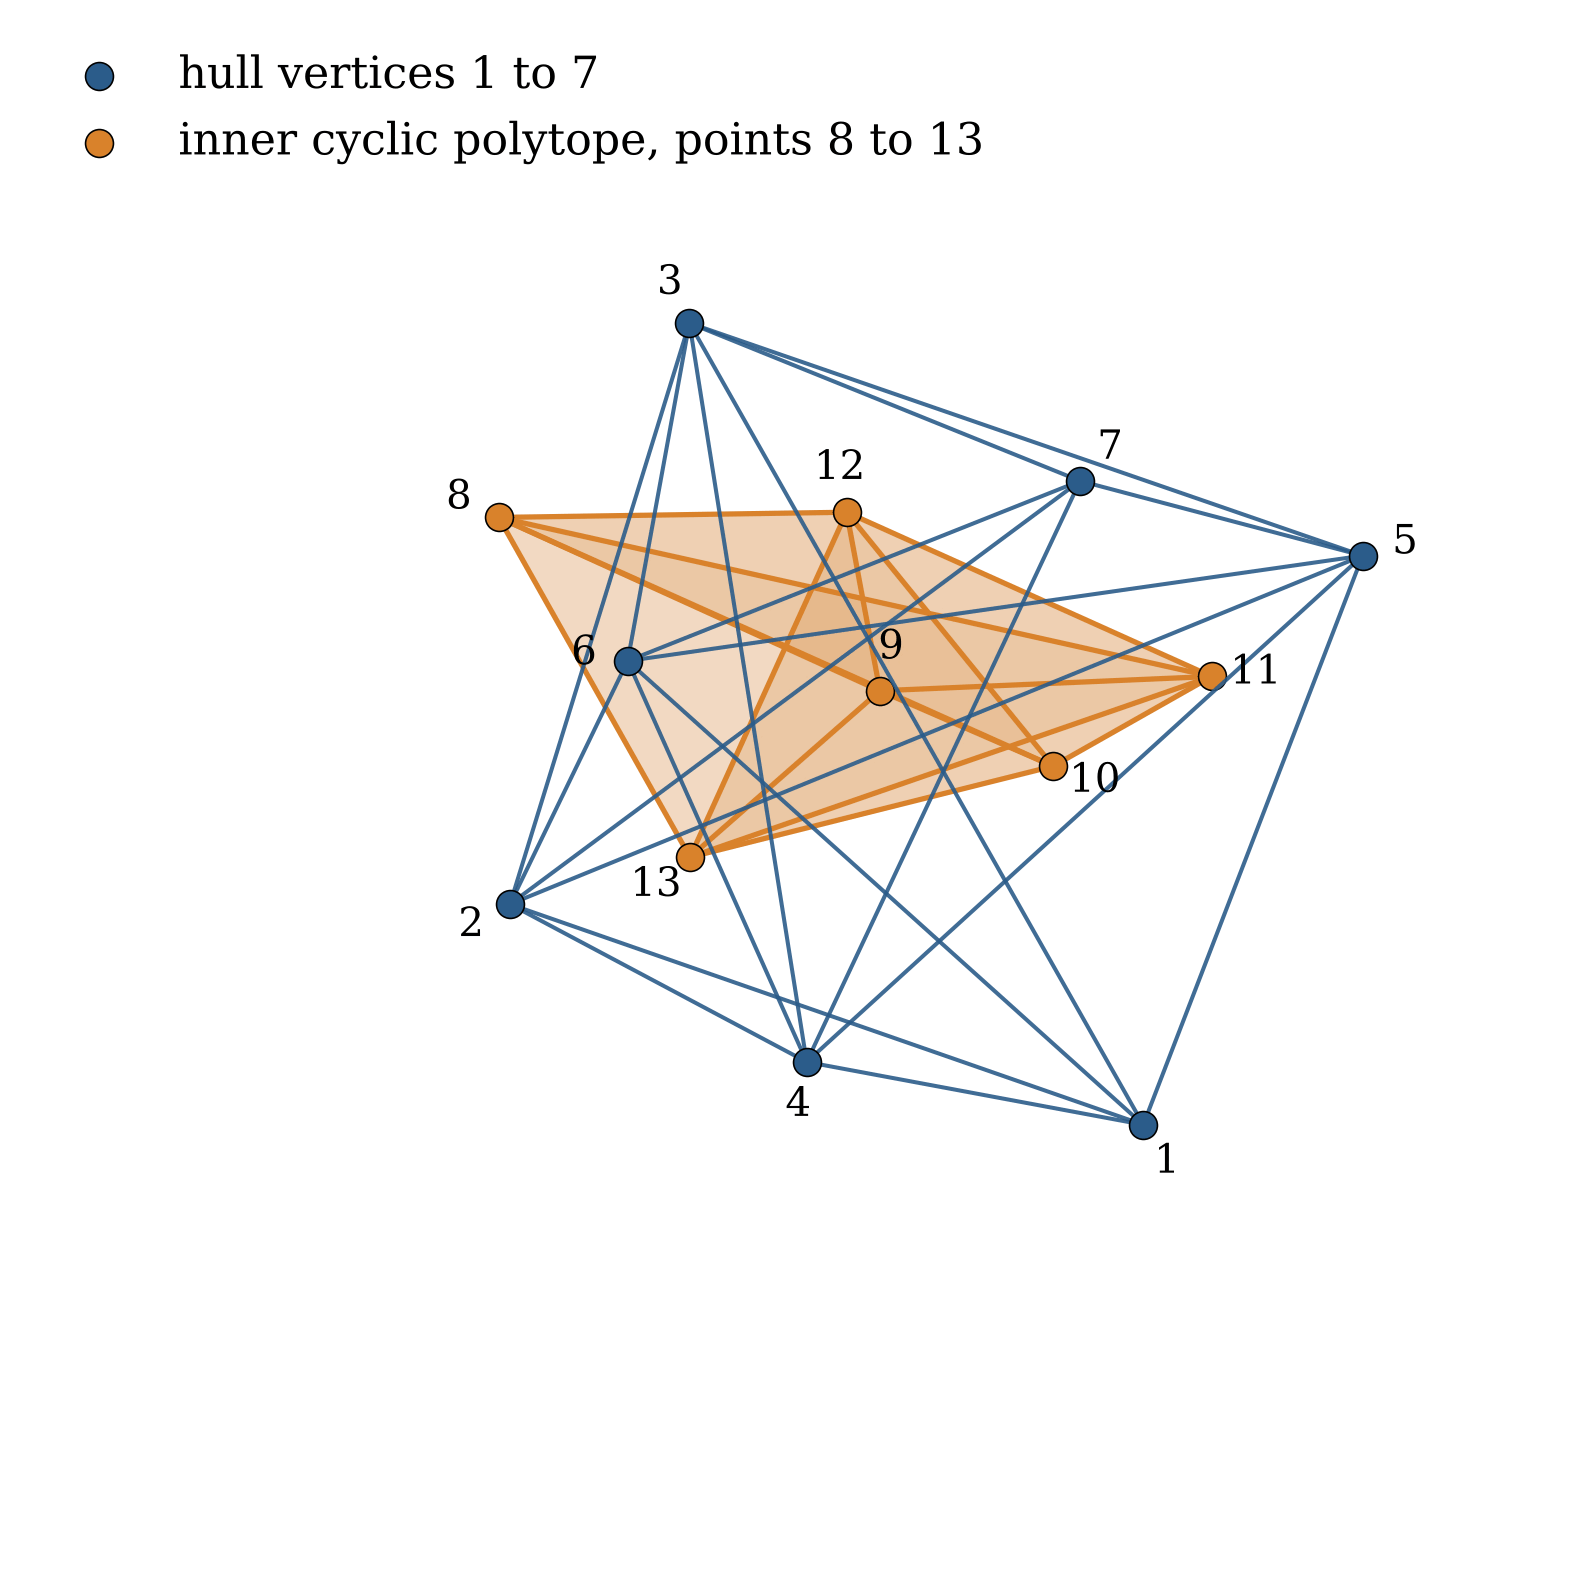
\includegraphics[width=\linewidth]{figures/fig_ninefour.png}
\caption{The thirteen points of Theorem~\ref{thm:C} in $\R^4$, after an affine map that makes the hull round and an orthogonal projection to $\R^3$ chosen to keep the points apart; the six inner points are drawn enlarged about their centre. Blue lines are the edges of the hull, which contain every pair of vertices except $x_1,x_7$; the orange polytope is the inner cyclic polytope $C_4(6)$.}\label{fig:ninefour}
\end{minipage}\hfill
\begin{minipage}[t]{0.485\textwidth}\centering
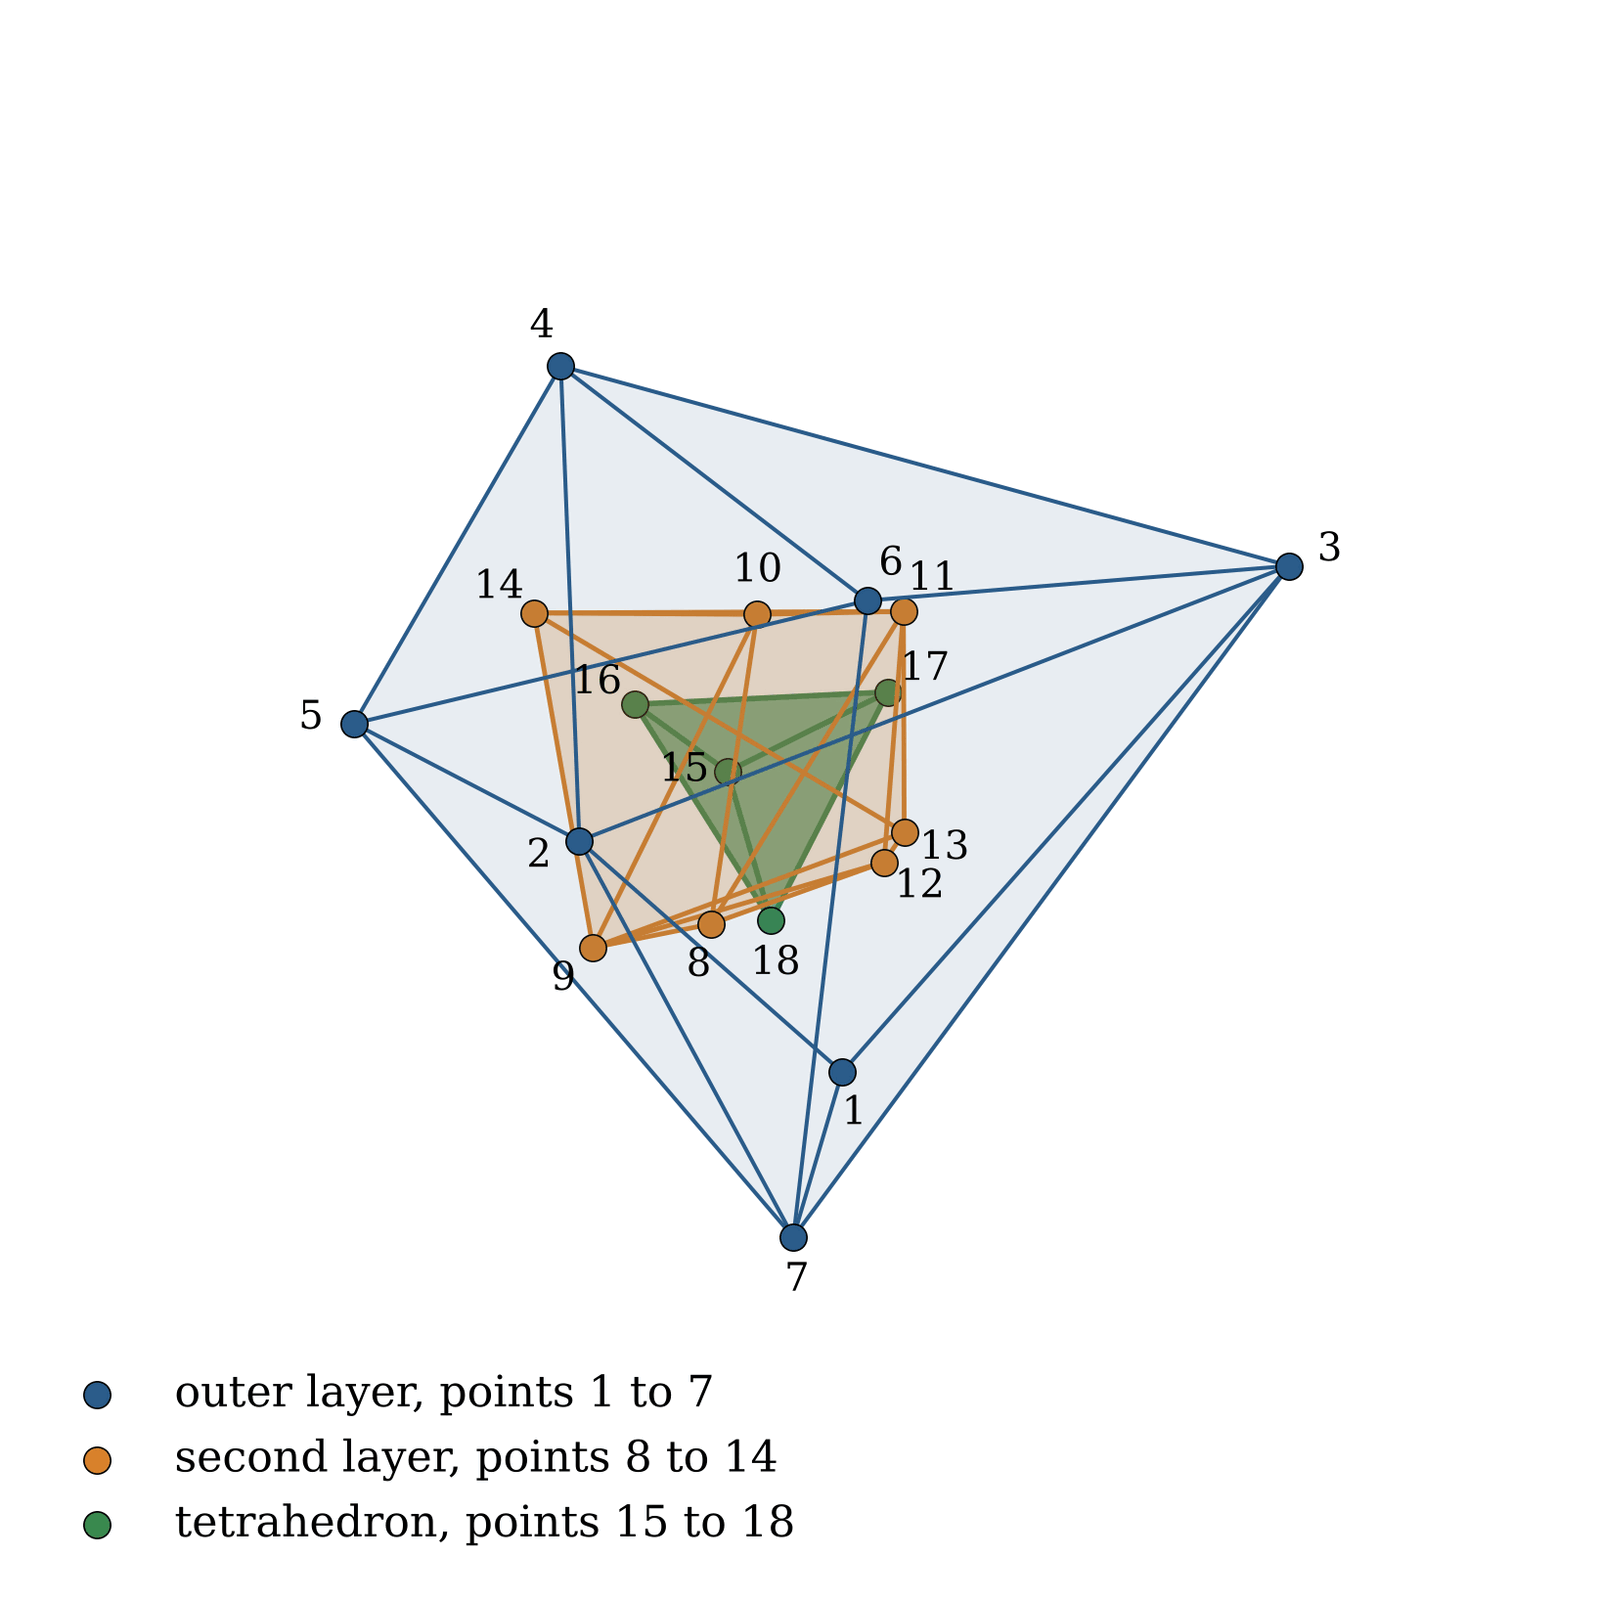
\includegraphics[width=\linewidth]{figures/fig_ninethree.png}
\caption{The three convex layers of the eighteen points of Theorem~\ref{thm:C} in $\R^3$: a capped octahedron (blue), a pentagonal bipyramid (orange) and a tetrahedron (green). Each layer is drawn after its own affine map and the layers are nested about a common centre, so the picture shows the true combinatorics and labels but not the true sizes.}\label{fig:ninethree}
\end{minipage}
\end{figure*}

\begin{proof}[Proof of Theorem~\ref{thm:C}]
Each row of Table~\ref{tab:certCfour} is a relation of $Y_4$, by the three checks of the proof of Theorem~\ref{thm:A}. Every one of the $\binom{13}{4}=715$ four-element subsets of the indices lies in one of the $\relCfour$ seven-element sets of the last column, so every $9$-subset of $Y_4$ contains the support of a relation, and $Y_4$ has no $9$ points in convex position by Proposition~\ref{prop:cover}. Its $\binom{13}{5}=1287$ determinants are nonzero, the smallest in absolute value being $\mindetCfour$. Each row of Tables~\ref{tab:certCthree} to~\ref{tab:certCthreec} is a relation of $Y_3$, and every one of the $\binom{18}{9}=48620$ subsets of size nine contains the support of one of these $\relCthree$ relations; this is verified as for Theorem~\ref{thm:B}, together with a direct test of every $9$-subset for convex position. The $\binom{18}{4}=3060$ determinants of $Y_3$ are nonzero, the smallest being $\mindetCthree$. Hence $g^{(4)}(9)\ge14$ and $g^{(3)}(9)\ge19$; holes are gons, so the same bounds hold for $h^{(4)}(9)$ and $h^{(3)}(9)$, and monotonicity gives $g^{(3)}(10)\ge20$.
\end{proof}

As before, the outer layer takes no part as the point $p$: every relation of $Y_4$ places one of $x_8,\dots,x_{13}$ inside a simplex, and every relation of $Y_3$ one of $x_8,\dots,x_{18}$, a vertex of the tetrahedron in $\relCthreeinner$ of the $\relCthree$ relations. A $9$-subset of $Y_4$ contains at least two of the six points of the cyclic polytope, and a $9$-subset of $Y_3$ at least two points of the two inner layers.

%----------------------------------------------------------------------
\section{How the sets were found}\label{sec:search}

The sets were found by local search over coordinates. For a candidate set we counted its $k$-subsets in convex position, but a bare count gives the search nothing to follow, since most moves change it by zero. We therefore scored each $k$-subset $Y$ by how far it is from failing: for every point $p$ of $Y$ and every simplex $\sigma$ of other points of $Y$, the least barycentric coordinate of $p$ with respect to $\sigma$ measures how far $p$ is from being inside, and the score of $Y$ is $f$ of the smallest such violation over $p$ and $\sigma$, with $f(t)=t/(1+t)$ for violations and $0$ for subsets that already fail. The total score is zero exactly for sets without $k$-gons. Simulated annealing on this score, with occasional \emph{repair moves} that take a point of a surviving $k$-gon and place it just inside the simplex of the subset nearest to it, found the eleven points in $\R^4$ and the fifteen points in $\R^3$, and for $k=9$ the thirteen points in $\R^4$ and the eighteen points in $\R^3$.\footnote{Before these constructions we checked the status of the problem in the literature cited here and with the BLLM engine Anaxia \cite{Ana26}. The engine keeps indexes of DeepMind's formal-conjectures collection and AlphaEvolve problem repository, of the OpenRefute archive and of OpenAI's collection of mathematical manuscripts, and answers a query with the matching entries and their recorded status. For the Erd\H{o}s--Szekeres problem these indexes hold only the planar question (Erd\H{o}s problem~107 in the formal-conjectures collection and problem~58 of the AlphaEvolve repository) and no entry on $g^{(d)}(k)$ for $d\ge3$, which agreed with our reading of \cite{Sch23} and of the papers citing it. The point sets of this paper were found and verified by the search and certificate programs of the archive \cite{BB26z}, not by the engine. The methods that found them, a graded count of violated subsets, repair moves that push a point just inside its nearest simplex, and the polishing of the least barycentric coordinate described below, were afterwards added to the engine as construction rules.}

The sets so found have real coordinates and some relations with very small barycentric coordinates. We then \emph{polished} each set by hill climbing on the least barycentric coordinate over a fixed certificate, which doubled it for the set in $\R^3$, and rounded to the coarsest integer grid on which a certificate survives; this gave coordinates at most $\maxcoordA$ and $\maxcoordCfour$ for the two sets in $\R^4$, and at most $\maxcoordB$ and $\maxcoordCthree$ for the two sets in $\R^3$. Finally we chose a certificate with few relations and small weights by a randomised greedy covering followed by removal of redundant relations. None of these steps is part of the proof.

%----------------------------------------------------------------------
\section{What remains open}\label{sec:open}

The value of $g^{(4)}(8)$ is now $12$ or $13$. The same search, run on twelve points in $\R^4$, ended with sets that still contain four $8$-gons, and twelve points in $\R^5$ without a $9$-gon ended at three $9$-gons; for fifteen points in $\R^3$ the search reached zero, while sixteen points ended at four $8$-gons. Scheucher's twelve-element chirotopes without $8$-gons and $9$-gons in rank five and six are not realizable either. A twelve-point set in $\R^4$ without an $8$-gon would prove $g^{(4)}(8)=13$ and confirm both conjectures quoted in the introduction; a proof that every twelve points contain an $8$-gon would refute them.

In three dimensions the gap is wider: $16\le g^{(3)}(8)$, while the conjectured value is $21$. The layered structure of $X_3$ suggests adding a fourth layer inside the tetrahedron or replacing the tetrahedron by a larger polytope. The value of $h^{(3)}(8)$ is not even known to be finite \cite{Sch23}.

For nine points the bounds are $14\le g^{(4)}(9)$ and $19\le g^{(3)}(9)$, against the conjectured $17$ and $33$. The search, run on fourteen points in $\R^4$ and on nineteen points in $\R^3$, ended with sets that still contain $4$ and $12$ subsets of nine points in convex position, and adding one point to the sets of Theorem~\ref{thm:C} at any of the $123450$ and $51591$ sampled positions left at least nine and eight such subsets.

Finally, the certificates are longer than the bounds of Remark~\ref{rem:schoenheim}: $\relA$ relations against $18$ and $\relCfour$ against $26$ in $\R^4$, and $\relB$ against $74$ and $\relCthree$ against $85$ in $\R^3$. In both sets the points $p$ of the relations are confined to the inner layers, so the supports are not spread evenly over the set, as a covering design meeting Sch\"onheim's bound would require.

%----------------------------------------------------------------------
\section*{Data and code availability}
The coordinates, the certificates, the search, polishing and rounding programs, the independent checks in Python, C, C++ and Julia, the Lean~4 file that checks all four certificates in the kernel, the figure programs and the \LaTeX{} source are in the repository \codeDOI{} and its Zenodo archive\zenodoDOI{} \cite{BB26z}. The status check of the problem was made with the BLLM engine Anaxia, release v3.0.5 \cite{Ana26}. Deep Bhattacharjee carried out the computations and the Python, C, C++, Julia, Lean and shell verifications with AI assistance (Claude, Anthropic).

\section*{Ethical declarations}
Funding: none. Competing interests: none.

\section*{Author contributions}
Deep Bhattacharjee proposed the problem, carried out the searches and computations and wrote the paper. Ushashi Bhattacharya checked the relations of Tables~\ref{tab:certA} and~\ref{tab:certCfour} and the proofs of Appendix~\ref{app:proofs}. Both authors approved the final version.

\appendix

%----------------------------------------------------------------------
\section{Proofs of the lemmas}\label{app:proofs}


\emph{Barycentric coordinates.} Let $v_0,\dots,v_d\in\R^d$ with $D=\det(v_0,\dots,v_d)\ne0$. For a point $p$ the system $\sum_j\lambda_j=1$, $\sum_j\lambda_jv_j=p$ has the matrix whose columns are $(1,v_j)$, the transpose of the matrix defining $D$, so it has the unique solution
\begin{equation}\label{eq:cramer}
\lambda_j=\frac{\det(v_0,\dots,v_{j-1},p,v_{j+1},\dots,v_d)}{D}
\end{equation}
by Cramer's rule. The point $p$ lies in the interior of $\conv\{v_0,\dots,v_d\}$ if and only if all $\lambda_j>0$: the simplex is the set where all $\lambda_j\ge0$, and its boundary is where some $\lambda_j=0$. Summing \eqref{eq:cramer} gives $\sum_j\det(v_0,\dots,p,\dots,v_d)=D$, an identity used to check tables: the numerators of a relation are $m_jD/M$ and add up to $D$.

\emph{Proof of the divisibility in Lemma~\ref{lem:interior}.} From $\lambda_j=m_j/M$ and \eqref{eq:cramer}, $m_jD=MN_j$ with $N_j$ the integer numerator. Choose integers $a_j$ with $\sum_ja_jm_j=1$. Then $D=\sum_ja_jm_jD=M\sum_ja_jN_j$.

\emph{An explicit $\varepsilon$ in Lemma~\ref{lem:stable}.} Let all $d+2$ points lie in a ball of radius $R\ge1$ around the origin and let $\delta=\min_j m_j/M$. The determinant $\det(v_0,\dots,v_d)$ is a multilinear function of the rows $(1,v_j)$. Moving each point by at most $\varepsilon\le R$ changes each row by at most $\varepsilon$ and keeps every row of norm at most $\sqrt{1+4R^2}\le3R$. Replacing the rows one at a time and applying Hadamard's inequality to each difference, the determinant changes by at most $(d+1)\,\varepsilon\,(3R)^{d}$, and the same holds for each numerator in \eqref{eq:cramer}. If $\varepsilon\le|D|\,\delta/\bigl(4(d+1)(3R)^d\bigr)$, then the new determinant has the sign of $D$ and modulus at least $\tfrac34|D|$, each new numerator differs from the old one $\lambda_jD$ by at most $\tfrac14\delta|D|$, and so every new barycentric coordinate is at least $\frac34\delta/\frac54=\frac35\delta>0$.

\emph{The general position claim of Proposition~\ref{prop:cover}.} Each $\det(x_{i_0},\dots,x_{i_d})$ is a polynomial in the $d|X|$ coordinates that does not vanish identically, since it is nonzero on any set of $d+1$ affinely independent points. A finite union of zero sets of nonzero polynomials has empty interior, so every neighbourhood of a configuration contains configurations in general position.

\emph{Sch\"onheim's bound.} A family of $s$-subsets of an $n$-set covering every $t$-subset has at least $\lceil\frac{n}{s}\lceil\frac{n-1}{s-1}\cdots\lceil\frac{n-t+1}{s-t+1}\rceil\cdots\rceil\rceil$ members \cite{Sch64}: the members containing a fixed point, with that point removed, cover all $(t-1)$-subsets of the remaining $n-1$ points, and counting incidences gives the recursion. For $(n,s,t)=(11,5,3)$ the bound is $\lceil\frac{11}{5}\lceil\frac{10}{4}\cdot3\rceil\rceil=\lceil\frac{11\cdot8}{5}\rceil=18$; for $(15,10,7)$ the nested values are $3,6,11,19,31,49,74$. For $k=9$ the thirteen points in $\R^4$ give $(n,s,t)=(13,7,4)$, with nested values $3,7,14,26$, and the eighteen points in $\R^3$ give $(18,13,9)$, with nested values $2,4,7,12,19,29,43,61,85$.

%----------------------------------------------------------------------
\section{The certificates}\label{app:certA}\label{app:certB}

Table~\ref{tab:certA} lists the $\relA$ relations of $X_4$, Tables~\ref{tab:certB} and~\ref{tab:certBb} the $\relB$ relations of $X_3$, Table~\ref{tab:certCfour} the $\relCfour$ relations of $Y_4$, and Tables~\ref{tab:certCthree} to~\ref{tab:certCthreec} the $\relCthree$ relations of $Y_3$, each ordered by $p$ and then by $\sigma$. The weights are the integers $m_j=M\lambda_j$ with $\gcd(m_0,\dots,m_d)=1$; the largest $M$ is $\maxMA$ for $X_4$, $\maxMB$ for $X_3$, $\maxMCfour$ for $Y_4$ and $\maxMCthree$ for $Y_3$. To check a row, multiply each point $x_{s_j}$ by $m_j$, add, and compare with $Mx_p$ coordinate by coordinate; then compute one determinant of size $d+1$, whose absolute value must be $gM$.

%----------------------------------------------------------------------
\begin{thebibliography}{99}\rightskip=0pt plus 3em

\bibitem{ES35} P.~Erd\H{o}s and G.~Szekeres, A combinatorial problem in geometry, \emph{Compositio Math.} \textbf{2} (1935), 463--470, \url{http://www.numdam.org/item/CM_1935__2__463_0/}.

\bibitem{MS00} W.~Morris and V.~Soltan, The Erd\H{o}s--Szekeres problem on points in convex position---a survey, \emph{Bull. Amer. Math. Soc.} \textbf{37} (2000), 437--458, \href{https://doi.org/10.1090/S0273-0979-00-00877-6}{doi:10.1090/S0273-0979-00-00877-6}.

\bibitem{SP06} G.~Szekeres and L.~Peters, Computer solution to the 17-point Erd\H{o}s--Szekeres problem, \emph{ANZIAM J.} \textbf{48} (2006), 151--164, \href{https://doi.org/10.1017/S144618110000300X}{doi:10.1017/S144618110000300X}.

\bibitem{Mar19} F.~Mari\'c, Fast formal proof of the Erd\H{o}s--Szekeres conjecture for convex polygons with at most 6 points, \emph{J. Automat. Reason.} \textbf{62} (2019), 301--329, \href{https://doi.org/10.1007/s10817-017-9423-7}{doi:10.1007/s10817-017-9423-7}.

\bibitem{Suk17} A.~Suk, On the Erd\H{o}s--Szekeres convex polygon problem, \emph{J. Amer. Math. Soc.} \textbf{30} (2017), 1047--1053, \href{https://doi.org/10.1090/jams/869}{doi:10.1090/jams/869}.

\bibitem{HS24} M.~J.~H.~Heule and M.~Scheucher, Happy ending: an empty hexagon in every set of 30 points, in \emph{Tools and Algorithms for the Construction and Analysis of Systems (TACAS 2024)}, Lecture Notes in Comput. Sci. \textbf{14570}, Springer, 2024, 61--80, \href{https://doi.org/10.1007/978-3-031-57246-3_5}{doi:10.1007/978-3-031-57246-3\_5}.

\bibitem{Sch23} M.~Scheucher, A SAT attack on Erd\H{o}s--Szekeres numbers in $\R^d$ and the empty hexagon theorem, \emph{Comput. Geom. Topol.} \textbf{2}(1) (2023), Article~2, 1--13, \href{https://doi.org/10.57717/cgt.v2i1.12}{doi:10.57717/cgt.v2i1.12}.

\bibitem{Kar01} G.~K\'arolyi, Ramsey-remainder for convex sets and the Erd\H{o}s--Szekeres theorem, \emph{Discrete Appl. Math.} \textbf{109} (2001), 163--175, \href{https://doi.org/10.1016/S0166-218X(00)00234-1}{doi:10.1016/S0166-218X(00)00234-1}.

\bibitem{KV03} G.~K\'arolyi and P.~Valtr, Point configurations in $d$-space without large subsets in convex position, \emph{Discrete Comput. Geom.} \textbf{30} (2003), 277--286, \href{https://doi.org/10.1007/s00454-003-0009-4}{doi:10.1007/s00454-003-0009-4}.

\bibitem{PZ25} C.~Pohoata and D.~Zakharov, Convex polytopes from fewer points, \emph{Duke Math. J.} \textbf{174} (2025), 449--471, \href{https://doi.org/10.1215/00127094-2024-0034}{doi:10.1215/00127094-2024-0034}.

\bibitem{Val92} P.~Valtr, Sets in $\R^d$ with no large empty convex subsets, \emph{Discrete Math.} \textbf{108} (1992), 115--124, \href{https://doi.org/10.1016/0012-365X(92)90665-3}{doi:10.1016/0012-365X(92)90665-3}.

\bibitem{DGK63} L.~Danzer, B.~Gr\"unbaum and V.~Klee, Helly's theorem and its relatives, in \emph{Convexity}, Proc. Sympos. Pure Math. \textbf{7}, Amer. Math. Soc., 1963, 101--180, \href{https://doi.org/10.1090/pspum/007/0157289}{doi:10.1090/pspum/007/0157289}.

\bibitem{BH95} T.~Bisztriczky and H.~Harborth, On empty convex polytopes, \emph{J. Geom.} \textbf{52} (1995), 25--29, \href{https://doi.org/10.1007/BF01406823}{doi:10.1007/BF01406823}.

\bibitem{BS94} T.~Bisztriczky and V.~Soltan, Some Erd\H{o}s--Szekeres type results about points in space, \emph{Monatsh. Math.} \textbf{118} (1994), 33--40, \href{https://doi.org/10.1007/BF01305772}{doi:10.1007/BF01305772}.

\bibitem{Sch64} J.~Sch\"onheim, On coverings, \emph{Pacific J. Math.} \textbf{14} (1964), 1405--1411, \href{https://doi.org/10.2140/pjm.1964.14.1405}{doi:10.2140/pjm.1964.14.1405}.

\bibitem{Zie95} G.~M.~Ziegler, \emph{Lectures on Polytopes}, Grad. Texts in Math. \textbf{152}, Springer, 1995, \href{https://doi.org/10.1007/978-1-4613-8431-1}{doi:10.1007/978-1-4613-8431-1}.

\bibitem{Gru03} B.~Gr\"unbaum, \emph{Convex Polytopes}, 2nd ed., Grad. Texts in Math. \textbf{221}, Springer, 2003, \href{https://doi.org/10.1007/978-1-4613-0019-9}{doi:10.1007/978-1-4613-0019-9}.

\bibitem{BBB26a} D.~Bhattacharjee, U.~Bhattacharya and S.~Bhattacharya, The sphere packing problem in dimension 4, \emph{Preprints} (2026), \href{https://doi.org/10.20944/preprints202606.0856.v11}{doi:10.20944/preprints202606.0856.v11}.

\bibitem{BBB26b} D.~Bhattacharjee, U.~Bhattacharya and S.~Bhattacharya, The sphere packing problem in dimension 7, \emph{Preprints} (2026), \href{https://doi.org/10.20944/preprints202606.1534.v9}{doi:10.20944/preprints202606.1534.v9}.

\bibitem{Bha26} D.~Bhattacharjee, Seed universality for reflexive polytopes in dimension four: generation of the Kreuzer--Skarke Calabi--Yau landscape via toric seed orbits, \emph{Preprints} (2026), \href{https://doi.org/10.20944/preprints202603.1056.v1}{doi:10.20944/preprints202603.1056.v1}.

\bibitem{Ana26} D.~Bhattacharjee and U.~Bhattacharya, Anaxia, the BLLM engine: verifier-gated conjecture closure, release v3.0.5 (2026), \href{https://doi.org/10.5281/zenodo.23469389}{doi:10.5281/zenodo.23469389} (all versions \href{https://doi.org/10.5281/zenodo.23286641}{doi:10.5281/zenodo.23286641}), with the paper \emph{BLLM: Beyond the LLM with Deep Human-Mind-AI}, \url{https://github.com/creelie/eBLLM}.

\bibitem{BB26z} D.~Bhattacharjee and U.~Bhattacharya, New lower bounds for Erd\H{o}s--Szekeres numbers in three and four dimensions: coordinates, certificates and checks, repository \url{https://github.com/creelie/Erdos-s1}, release v1.1.0 (2026)\zenodoDOI.

\end{thebibliography}

\clearpage
\begin{table*}[tp]
\caption{The twenty-eight relations behind Theorem~\ref{thm:A}. In each row the point $x_p$ satisfies $\sum_j m_j x_{s_j}=M x_p$ with $\sigma=\{s_1,\dots,s_5\}$ listed in increasing order, the weights $m_j$ are positive integers with sum $M$, and $|\det\sigma|=gM$ for the $5\times5$ determinant of the rows $(1,x_s)$, $s\in\sigma$. The last column lists the five points not used by the relation; every triple of $\{1,\dots,11\}$ lies in one of these sets.}\label{tab:certA}
\begin{ruledtabular}
\begin{tabular}{rlrrrrrrrl}
$p$ & $\sigma$ & $m_1$ & $m_2$ & $m_3$ & $m_4$ & $m_5$ & $M$ & $g$ & unused points \\ \hline
7 & 1,2,3,4,10 & 7673 & 6278 & 15495 & 2902 & 10393 & 42741 & 9 & 5,6,8,9,11 \\
7 & 1,2,3,6,11 & 1878 & 304 & 1910 & 74 & 2217 & 6383 & 3 & 4,5,8,9,10 \\
7 & 1,3,4,8,9 & 30287 & 42693 & 6085 & 50075 & 3654 & 132794 & 1 & 2,5,6,10,11 \\
7 & 1,3,6,8,11 & 614 & 550 & 194 & 152 & 297 & 1807 & 6 & 2,4,5,9,10 \\
8 & 1,2,3,6,10 & 1410 & 2694 & 598 & 3109 & 4628 & 12439 & 9 & 4,5,7,9,11 \\
8 & 1,2,5,6,7 & 44866 & 11396 & 12870 & 62375 & 5226 & 136733 & 1 & 3,4,9,10,11 \\
8 & 1,2,5,6,9 & 9820 & 2570 & 1833 & 13526 & 2613 & 30362 & 2 & 3,4,7,10,11 \\
8 & 1,2,5,10,11 & 2589 & 9511 & 2031 & 3027 & 22996 & 40154 & 1 & 3,4,6,7,9 \\
8 & 1,2,9,10,11 & 723 & 6103 & 2031 & 3933 & 11728 & 24518 & 1 & 3,4,5,6,7 \\
8 & 2,3,4,5,11 & 6507 & 1387 & 3142 & 3765 & 3887 & 18688 & 9 & 1,6,7,9,10 \\
8 & 2,3,6,10,11 & 3114 & 328 & 109 & 3458 & 4230 & 11239 & 3 & 1,4,5,7,9 \\
8 & 2,4,5,9,11 & 11222 & 3936 & 1011 & 12483 & 11060 & 39712 & 1 & 1,3,6,7,10 \\
8 & 2,4,6,7,10 & 1990 & 104 & 1315 & 1442 & 3186 & 8037 & 18 & 1,3,5,9,11 \\
8 & 2,7,9,10,11 & 1380 & 241 & 228 & 1214 & 2219 & 5282 & 3 & 1,3,4,5,6 \\
9 & 1,3,5,6,11 & 19212 & 13094 & 38497 & 14620 & 12438 & 97861 & 1 & 2,4,7,8,10 \\
9 & 1,5,6,7,10 & 1198 & 19329 & 4916 & 23140 & 2066 & 50649 & 1 & 2,3,4,8,11 \\
9 & 2,3,4,5,7 & 1574 & 1628 & 1448 & 6753 & 3144 & 14547 & 12 & 1,6,8,10,11 \\
9 & 2,3,4,5,10 & 14378 & 20588 & 3032 & 37755 & 37728 & 113481 & 1 & 1,6,7,8,11 \\
9 & 2,3,5,7,11 & 290 & 104 & 4493 & 4616 & 2172 & 11675 & 8 & 1,4,6,8,10 \\
9 & 3,5,7,8,10 & 1726 & 6667 & 3702 & 5104 & 2392 & 19591 & 1 & 1,2,4,6,11 \\
10 & 1,4,5,6,9 & 14386 & 23140 & 33623 & 3752 & 9577 & 84478 & 1 & 2,3,7,8,11 \\
10 & 1,4,5,7,8 & 14270 & 30691 & 47880 & 6133 & 10247 & 109221 & 1 & 2,3,6,9,11 \\
10 & 1,4,5,9,11 & 4022 & 5844 & 9829 & 11 & 3752 & 23458 & 1 & 2,3,6,7,8 \\
11 & 1,3,4,6,10 & 3149 & 4165 & 2999 & 16899 & 15406 & 42618 & 6 & 2,5,7,8,9 \\
11 & 1,4,6,7,9 & 16 & 898 & 1756 & 853 & 2136 & 5659 & 13 & 2,3,5,8,10 \\
11 & 3,4,6,7,10 & 608 & 1150 & 5848 & 3149 & 5748 & 16503 & 6 & 1,2,5,8,9 \\
11 & 3,4,6,8,9 & 5074 & 16942 & 25719 & 14465 & 36606 & 98806 & 1 & 1,2,5,7,10 \\
11 & 4,5,6,7,10 & 280 & 228 & 686 & 639 & 166 & 1999 & 16 & 1,2,3,8,9 \\
\end{tabular}
\end{ruledtabular}
\end{table*}

\begin{table*}[tp]
\scriptsize
\caption{The 161 relations behind Theorem~\ref{thm:B}. Each row gives $\sum_j m_j x_{s_j}=M x_p$ with $\sigma=\{s_1,\dots,s_4\}$ in increasing order, positive integer weights $m_j$ with sum $M$, and $|\det\sigma|=gM$ for the $4\times4$ determinant of the rows $(1,x_s)$.}\label{tab:certB}
\begin{ruledtabular}
\begin{tabular}{rlrrrrrr@{\hspace{2.2em}}rlrrrrrr}
$p$ & $\sigma$ & $m_1$ & $m_2$ & $m_3$ & $m_4$ & $M$ & $g$ & $p$ & $\sigma$ & $m_1$ & $m_2$ & $m_3$ & $m_4$ & $M$ & $g$ \\ \hline
6 & 1,2,3,12 & 1939 & 18838 & 7809 & 46242 & 74828 & 3 & 9 & 3,4,10,14 & 88 & 1 & 49 & 6 & 144 & 24 \\
6 & 1,2,10,11 & 9628 & 26527 & 16482 & 12471 & 65108 & 16 & 9 & 3,4,14,15 & 383 & 192 & 25 & 98 & 698 & 12 \\
6 & 2,3,4,8 & 34648 & 2701 & 12313 & 31010 & 80672 & 1 & 9 & 3,5,10,13 & 17959 & 6 & 10191 & 1152 & 29308 & 3 \\
6 & 2,3,7,9 & 37155 & 8333 & 10899 & 22519 & 78906 & 1 & 9 & 3,7,10,12 & 25061 & 516 & 13953 & 306 & 39836 & 2 \\
6 & 2,3,10,13 & 18392 & 4499 & 2471 & 15911 & 41273 & 2 & 9 & 3,8,10,13 & 3029 & 18 & 1725 & 168 & 4940 & 1 \\
6 & 2,4,8,15 & 44768 & 15282 & 42383 & 2701 & 105134 & 1 & 10 & 2,4,5,9 & 843 & 67592 & 2067 & 6503 & 77005 & 8 \\
6 & 2,4,9,14 & 22436 & 853 & 4834 & 22793 & 50916 & 1 & 10 & 2,4,5,14 & 688 & 155085 & 5760 & 13006 & 174539 & 4 \\
6 & 2,4,11,13 & 23569 & 922 & 1769 & 29068 & 55328 & 6 & 10 & 3,4,6,11 & 102 & 2399 & 8 & 164 & 2673 & 78 \\
6 & 2,5,7,13 & 11252 & 894 & 3044 & 10945 & 26135 & 4 & 10 & 4,5,6,7 & 66389 & 3431 & 678 & 5263 & 75761 & 4 \\
6 & 2,7,8,12 & 6744 & 757 & 4793 & 13076 & 25370 & 2 & 10 & 4,5,6,15 & 58359 & 1525 & 1234 & 5263 & 66381 & 4 \\
6 & 2,7,8,15 & 20536 & 7641 & 4885 & 13076 & 46138 & 2 & 10 & 4,5,8,12 & 15380 & 550 & 941 & 151 & 17022 & 16 \\
6 & 2,8,9,13 & 9620 & 98 & 3784 & 8101 & 21603 & 1 & 10 & 4,5,11,13 & 15563 & 364 & 492 & 1144 & 17563 & 5 \\
6 & 2,8,10,14 & 162 & 110 & 49 & 59 & 380 & 33 & 10 & 4,7,9,11 & 22967 & 156 & 1352 & 1668 & 26143 & 2 \\
6 & 2,8,12,13 & 1388 & 590 & 1892 & 757 & 4627 & 2 & 10 & 4,8,11,15 & 17657 & 104 & 1076 & 1196 & 20033 & 2 \\
6 & 2,8,12,14 & 1732 & 337 & 1617 & 1514 & 5200 & 1 & 10 & 4,11,14,15 & 3123 & 192 & 26 & 208 & 3549 & 8 \\
6 & 2,9,13,15 & 2088 & 676 & 1843 & 98 & 4705 & 1 & 11 & 1,3,5,12 & 265 & 7257 & 36613 & 35711 & 79846 & 4 \\
6 & 2,12,14,15 & 4536 & 1977 & 5036 & 337 & 11886 & 1 & 11 & 2,3,5,9 & 373 & 67 & 1019 & 829 & 2288 & 132 \\
7 & 1,2,4,14 & 4432 & 26 & 8779 & 2337 & 15574 & 28 & 11 & 2,4,5,14 & 22503 & 6553 & 82862 & 62621 & 174539 & 4 \\
7 & 1,3,4,10 & 678 & 10 & 151 & 1297 & 2136 & 8 & 11 & 2,5,6,9 & 541 & 13490 & 8844 & 6698 & 29573 & 1 \\
7 & 1,4,6,9 & 75367 & 143525 & 6344 & 27906 & 253142 & 1 & 11 & 2,5,6,15 & 21 & 323 & 194 & 197 & 735 & 34 \\
7 & 1,4,6,13 & 8006 & 15830 & 55 & 4651 & 28542 & 6 & 11 & 2,5,8,10 & 3511 & 13381 & 7879 & 3834 & 28605 & 28 \\
7 & 1,4,10,13 & 30 & 29 & 33 & 8 & 100 & 10 & 11 & 2,5,12,13 & 3067 & 23571 & 10347 & 12688 & 49673 & 2 \\
7 & 1,4,10,14 & 64 & 43 & 91 & 10 & 208 & 8 & 11 & 2,5,13,15 & 4723 & 14241 & 3298 & 10347 & 32609 & 2 \\
7 & 1,4,10,15 & 152 & 44 & 278 & 5 & 479 & 16 & 11 & 3,5,6,7 & 1676 & 83567 & 49814 & 30595 & 165652 & 1 \\
8 & 1,2,3,7 & 17633 & 28610 & 171431 & 22934 & 240608 & 2 & 11 & 3,5,8,12 & 826 & 4874 & 265 & 4683 & 10648 & 4 \\
8 & 1,2,3,13 & 20655 & 26750 & 157849 & 45868 & 251122 & 1 & 11 & 4,5,6,15 & 238 & 39299 & 28782 & 20189 & 88508 & 3 \\
8 & 1,2,3,15 & 11419 & 10214 & 51009 & 22934 & 95576 & 2 & 11 & 5,6,9,10 & 119571 & 88052 & 53191 & 541 & 261355 & 1 \\
8 & 1,2,5,10 & 66745 & 3274 & 41539 & 49561 & 161119 & 12 & 11 & 5,6,10,15 & 103633 & 75898 & 714 & 53191 & 233436 & 1 \\
8 & 1,3,6,9 & 2193 & 14585 & 5988 & 1030 & 23796 & 5 & 11 & 5,6,12,14 & 3785 & 1124 & 1749 & 1406 & 8064 & 5 \\
8 & 1,3,6,12 & 2616 & 17890 & 5176 & 2575 & 28257 & 2 & 11 & 5,8,12,15 & 11307 & 2407 & 9968 & 826 & 24508 & 4 \\
8 & 1,3,11,14 & 4523 & 2132 & 5932 & 9799 & 22386 & 4 & 12 & 1,2,4,5 & 3861 & 7214 & 8827 & 2875 & 22777 & 92 \\
8 & 1,5,6,13 & 24028 & 16925 & 4483 & 61335 & 106771 & 4 & 12 & 1,2,9,10 & 467 & 5591 & 7309 & 2418 & 15785 & 28 \\
8 & 1,5,7,11 & 3284 & 2091 & 4838 & 1964 & 12177 & 14 & 12 & 2,3,4,14 & 6064 & 3551 & 3779 & 4228 & 17622 & 4 \\
8 & 1,5,12,14 & 4225 & 2788 & 1263 & 10679 & 18955 & 16 & 12 & 2,4,7,11 & 4201 & 1046 & 6290 & 2977 & 14514 & 26 \\
8 & 1,7,11,15 & 646 & 205 & 748 & 861 & 2460 & 34 & 12 & 2,4,8,9 & 4886 & 2792 & 3343 & 3678 & 14699 & 4 \\
8 & 1,11,13,15 & 9778 & 10804 & 6970 & 11603 & 39155 & 1 & 12 & 2,4,8,15 & 16672 & 12154 & 16385 & 7356 & 52567 & 2 \\
9 & 1,3,4,5 & 1926 & 43091 & 24609 & 2082 & 71708 & 4 & 12 & 2,5,7,10 & 19372 & 6561 & 30758 & 4706 & 61397 & 10 \\
9 & 1,3,10,15 & 69 & 5116 & 3003 & 474 & 8662 & 4 & 12 & 2,8,10,11 & 28610 & 35593 & 28094 & 1370 & 93667 & 4 \\
9 & 3,4,5,14 & 14479 & 7377 & 294 & 1926 & 24076 & 4 & 12 & 2,9,10,13 & 17111 & 14023 & 6497 & 13076 & 50707 & 1 \\
9 & 3,4,7,15 & 1844 & 906 & 75 & 639 & 3464 & 4 & 12 & 2,9,10,14 & 3527 & 2265 & 1514 & 3269 & 10575 & 4 \\
9 & 3,4,8,11 & 1495 & 771 & 78 & 48 & 2392 & 32 & 12 & 2,10,13,15 & 26536 & 11836 & 29826 & 14023 & 82221 & 1 \\
\end{tabular}
\end{ruledtabular}
\end{table*}

\begin{table*}[tp]
\scriptsize
\caption{The relations behind Theorem~\ref{thm:B}, continued. Each row gives $\sum_j m_j x_{s_j}=M x_p$ with $\sigma=\{s_1,\dots,s_4\}$ in increasing order, positive integer weights $m_j$ with sum $M$, and $|\det\sigma|=gM$ for the $4\times4$ determinant of the rows $(1,x_s)$.}\label{tab:certBb}
\begin{ruledtabular}
\begin{tabular}{rlrrrrrr@{\hspace{2.2em}}rlrrrrrr}
$p$ & $\sigma$ & $m_1$ & $m_2$ & $m_3$ & $m_4$ & $M$ & $g$ & $p$ & $\sigma$ & $m_1$ & $m_2$ & $m_3$ & $m_4$ & $M$ & $g$ \\ \hline
12 & 3,4,6,15 & 64 & 468 & 2782 & 399 & 3713 & 8 & 14 & 1,7,9,11 & 107 & 492 & 410 & 262 & 1271 & 78 \\
12 & 4,5,6,7 & 8542 & 2774 & 55354 & 9091 & 75761 & 4 & 14 & 1,8,9,10 & 493 & 7390 & 1956 & 2944 & 12783 & 4 \\
12 & 4,5,6,13 & 9726 & 1279 & 54191 & 9091 & 74287 & 4 & 14 & 1,9,12,13 & 915 & 7412 & 1942 & 544 & 10813 & 1 \\
12 & 4,6,8,11 & 2174 & 9752 & 1251 & 416 & 13593 & 13 & 14 & 1,10,12,15 & 861 & 714 & 654 & 4012 & 6241 & 28 \\
12 & 4,6,9,11 & 1771 & 11336 & 1807 & 205 & 15119 & 9 & 14 & 2,3,7,15 & 1308 & 7224 & 8445 & 6181 & 23158 & 4 \\
12 & 4,6,13,15 & 1236 & 7742 & 128 & 1279 & 10385 & 4 & 14 & 2,3,11,13 & 68 & 1839 & 446 & 25292 & 27645 & 4 \\
12 & 5,6,9,10 & 657 & 196364 & 29492 & 34842 & 261355 & 1 & 14 & 3,4,7,8 & 639 & 1351 & 584 & 4262 & 6836 & 4 \\
12 & 6,7,10,11 & 96074 & 13359 & 17426 & 8176 & 135035 & 1 & 14 & 3,5,7,12 & 9500 & 1213 & 12690 & 4103 & 27506 & 4 \\
12 & 6,7,10,15 & 3492 & 73 & 626 & 511 & 4702 & 16 & 14 & 3,5,8,13 & 674 & 185 & 483 & 16388 & 17730 & 2 \\
12 & 6,8,10,15 & 3370 & 146 & 688 & 365 & 4569 & 8 & 14 & 3,6,7,15 & 6366 & 2616 & 7263 & 5047 & 21292 & 2 \\
12 & 6,9,10,11 & 29872 & 4453 & 5313 & 219 & 39857 & 3 & 14 & 3,6,9,13 & 3 & 1 & 2 & 29 & 35 & 366 \\
13 & 1,2,4,14 & 5485 & 1118 & 12107 & 199326 & 218036 & 2 & 14 & 3,8,10,13 & 143 & 526 & 185 & 1616 & 2470 & 2 \\
13 & 1,3,4,12 & 14660 & 62357 & 37121 & 29606 & 143744 & 2 & 14 & 3,8,13,15 & 18 & 171 & 1686 & 185 & 2060 & 2 \\
13 & 1,4,8,9 & 2617 & 14795 & 35938 & 5246 & 58596 & 1 & 14 & 3,12,13,15 & 168 & 57 & 1638 & 61 & 1924 & 6 \\
13 & 1,4,8,14 & 3 & 14 & 26 & 61 & 104 & 86 & 14 & 4,8,9,13 & 127 & 652 & 258 & 1580 & 2617 & 1 \\
13 & 1,6,10,14 & 1111 & 433 & 2612 & 34331 & 38487 & 4 & 14 & 5,7,8,15 & 153 & 1137 & 789 & 335 & 2414 & 8 \\
13 & 1,6,10,15 & 17930 & 9491 & 21574 & 68662 & 117657 & 2 & 14 & 7,8,9,10 & 986 & 4766 & 1250 & 1217 & 8219 & 2 \\
13 & 1,7,9,11 & 7247 & 46781 & 25215 & 19895 & 99138 & 1 & 14 & 7,8,9,11 & 4690 & 4173 & 2981 & 1217 & 13061 & 2 \\
13 & 1,7,12,15 & 2236 & 7328 & 3305 & 17285 & 30154 & 4 & 14 & 7,8,12,15 & 1113 & 1281 & 153 & 1465 & 4012 & 8 \\
13 & 1,9,10,11 & 32261 & 37064 & 46781 & 28706 & 144812 & 1 & 14 & 8,9,11,13 & 1133 & 1051 & 127 & 9380 & 11691 & 1 \\
13 & 2,3,7,11 & 5213 & 53574 & 110580 & 23621 & 192988 & 1 & 15 & 1,2,5,9 & 149 & 1025 & 2593 & 39087 & 42854 & 26 \\
13 & 2,7,8,15 & 816 & 16327 & 12479 & 16516 & 46138 & 2 & 15 & 1,5,9,12 & 102 & 1039 & 13976 & 1025 & 16142 & 26 \\
13 & 2,7,10,14 & 566 & 10230 & 707 & 102737 & 114240 & 1 & 15 & 1,9,11,12 & 269 & 85895 & 13507 & 615 & 100286 & 2 \\
13 & 3,5,7,12 & 8302 & 1144 & 14043 & 4017 & 27506 & 4 & 15 & 2,3,4,11 & 949 & 59735 & 28841 & 14709 & 104234 & 4 \\
13 & 3,7,8,10 & 28 & 95 & 291 & 100 & 514 & 52 & 15 & 2,5,9,14 & 927 & 2721 & 38973 & 1937 & 44558 & 2 \\
13 & 3,7,12,15 & 86 & 111 & 49 & 44 & 290 & 104 & 15 & 2,8,9,11 & 151 & 608 & 56698 & 8669 & 66126 & 2 \\
13 & 4,7,12,14 & 58 & 1771 & 309 & 17496 & 19634 & 2 & 15 & 3,4,5,7 & 2303 & 1039 & 866 & 1894 & 6102 & 16 \\
13 & 5,6,7,14 & 71 & 149 & 1557 & 11252 & 13029 & 4 & 15 & 3,4,5,13 & 9661 & 5505 & 2266 & 7576 & 25008 & 4 \\
13 & 5,7,8,9 & 335 & 2307 & 1104 & 68 & 3814 & 8 & 15 & 3,5,7,10 & 4024 & 1376 & 3031 & 2078 & 10509 & 8 \\
13 & 6,7,8,15 & 204 & 1783 & 1367 & 1780 & 5134 & 8 & 15 & 3,5,8,10 & 6597 & 1129 & 3031 & 5225 & 15982 & 8 \\
13 & 6,7,14,15 & 45 & 333 & 2734 & 71 & 3183 & 4 & 15 & 3,5,9,12 & 34 & 83 & 1188 & 97 & 1402 & 78 \\
13 & 7,8,9,12 & 3839 & 4183 & 5296 & 1340 & 14658 & 2 & 15 & 3,6,9,11 & 551 & 534 & 57097 & 8691 & 66873 & 1 \\
13 & 7,8,11,14 & 1051 & 215 & 192 & 4504 & 5962 & 1 & 15 & 3,10,11,12 & 38783 & 21151 & 8684 & 1618 & 70236 & 2 \\
13 & 7,11,12,14 & 1813 & 116 & 215 & 14582 & 16726 & 1 & 15 & 5,6,8,9 & 4157 & 3404 & 567 & 61068 & 69196 & 2 \\
14 & 1,2,7,15 & 7224 & 3180 & 17781 & 61453 & 89638 & 4 & 15 & 5,7,9,13 & 487 & 747 & 2788 & 394 & 4416 & 2 \\
14 & 1,3,5,10 & 5297 & 144 & 3022 & 8242 & 16705 & 16 & 15 & 5,9,12,14 & 399 & 5040 & 309 & 442 & 6190 & 6 \\
14 & 1,3,7,11 & 437 & 2665 & 7462 & 2802 & 13366 & 12 & 15 & 9,10,11,14 & 12492 & 3 & 2022 & 469 & 14986 & 2 \\
14 & 1,4,5,11 & 1731 & 2378 & 1066 & 32 & 5207 & 52 & 15 & 9,11,13,14 & 945 & 153 & 6 & 29 & 1133 & 1 \\
14 & 1,4,6,15 & 18987 & 15234 & 11388 & 94354 & 139963 & 2 &  &  &  &  &  &  &  &  \\
14 & 1,5,7,9 & 5041 & 10218 & 39908 & 332 & 55499 & 2 &  &  &  &  &  &  &  &  \\
14 & 1,5,13,15 & 288 & 225 & 12462 & 1207 & 14182 & 4 &  &  &  &  &  &  &  &  \\
\end{tabular}
\end{ruledtabular}
\end{table*}

\begin{table*}[tp]
\footnotesize
\caption{The forty-six relations behind Theorem~\ref{thm:C} in $\mathbb{R}^4$. In each row the point $x_p$ satisfies $\sum_j m_j x_{s_j}=M x_p$ with $\sigma=\{s_1,\dots,s_5\}$ listed in increasing order, the weights $m_j$ are positive integers with sum $M$, and $|\det\sigma|=gM$ for the $5\times5$ determinant of the rows $(1,x_s)$, $s\in\sigma$. The last column lists the seven points not used by the relation; every four-element subset of $\{1,\dots,13\}$ lies in one of these sets.}\label{tab:certCfour}
\begin{ruledtabular}
\begin{tabular}{rlrrrrrrrl}
$p$ & $\sigma$ & $m_1$ & $m_2$ & $m_3$ & $m_4$ & $m_5$ & $M$ & $g$ & unused points \\ \hline
8 & 1,2,3,9,12 & 1065 & 23360 & 32113 & 19634 & 1985 & 78157 & 2 & 4,5,6,7,10,11,13 \\
8 & 2,3,4,5,7 & 9823 & 12191 & 1729 & 1393 & 1807 & 26943 & 33 & 1,6,9,10,11,12,13 \\
8 & 2,3,5,12,13 & 5224 & 6205 & 1085 & 546 & 1599 & 14659 & 6 & 1,4,6,7,9,10,11 \\
8 & 2,3,9,10,11 & 1039 & 1367 & 565 & 218 & 108 & 3297 & 5 & 1,4,5,6,7,12,13 \\
9 & 1,2,7,8,10 & 584 & 25560 & 35635 & 12157 & 50487 & 124423 & 1 & 3,4,5,6,11,12,13 \\
9 & 2,3,5,6,10 & 30730 & 5384 & 38739 & 32805 & 9809 & 117467 & 3 & 1,4,7,8,11,12,13 \\
9 & 2,3,7,10,11 & 673 & 113 & 785 & 1171 & 76 & 2818 & 21 & 1,4,5,6,8,12,13 \\
9 & 2,4,5,7,12 & 1696 & 375 & 1009 & 891 & 2882 & 6853 & 38 & 1,3,6,8,10,11,13 \\
9 & 2,5,6,8,13 & 8995 & 14013 & 10234 & 5124 & 3611 & 41977 & 3 & 1,3,4,7,10,11,12 \\
9 & 2,7,8,11,12 & 9261 & 6002 & 499 & 15763 & 10039 & 41564 & 1 & 1,3,4,5,6,10,13 \\
10 & 1,2,5,6,12 & 29352 & 6810 & 35371 & 39580 & 56485 & 167598 & 2 & 3,4,7,8,9,11,13 \\
10 & 1,2,7,12,13 & 36023 & 4334 & 39646 & 73314 & 22703 & 176020 & 1 & 3,4,5,6,8,9,11 \\
10 & 1,3,4,7,11 & 1114 & 4885 & 8801 & 973 & 31221 & 46994 & 2 & 2,5,6,8,9,12,13 \\
10 & 1,3,5,6,9 & 18438 & 4996 & 22895 & 33055 & 19957 & 99341 & 5 & 2,4,7,8,11,12,13 \\
10 & 1,3,5,8,13 & 2127 & 1416 & 5224 & 318 & 13085 & 22170 & 20 & 2,4,6,7,9,11,12 \\
10 & 1,4,5,8,12 & 2158 & 5995 & 6094 & 2755 & 14915 & 31917 & 6 & 2,3,6,7,9,11,13 \\
10 & 1,4,11,12,13 & 349 & 126 & 1592 & 1234 & 315 & 3616 & 3 & 2,3,5,6,7,8,9 \\
10 & 1,6,7,9,12 & 15664 & 5931 & 14264 & 10135 & 25537 & 71531 & 1 & 2,3,4,5,8,11,13 \\
10 & 1,6,8,11,12 & 2161 & 2079 & 315 & 8987 & 3721 & 17263 & 3 & 2,3,4,5,7,9,13 \\
10 & 1,6,9,11,12 & 3832 & 3213 & 945 & 14264 & 7687 & 29941 & 1 & 2,3,4,5,7,8,13 \\
10 & 3,4,5,9,13 & 13629 & 27615 & 24194 & 12498 & 8815 & 86751 & 1 & 1,2,6,7,8,11,12 \\
11 & 1,2,3,6,7 & 4243 & 1170 & 1025 & 547 & 10331 & 17316 & 84 & 4,5,8,9,10,12,13 \\
11 & 1,2,3,7,10 & 29589 & 8801 & 6829 & 78800 & 22974 & 146993 & 2 & 4,5,6,8,9,12,13 \\
11 & 1,2,5,12,13 & 4791 & 4452 & 44731 & 21711 & 43349 & 119034 & 2 & 3,4,6,7,8,9,10 \\
11 & 1,3,7,9,12 & 23024 & 3663 & 51512 & 27931 & 3659 & 109789 & 1 & 2,4,5,6,8,10,13 \\
11 & 1,4,5,6,8 & 707 & 13603 & 36966 & 12587 & 15170 & 79033 & 3 & 2,3,7,9,10,12,13 \\
11 & 1,7,8,9,13 & 3925 & 9542 & 2180 & 1306 & 639 & 17592 & 4 & 2,3,4,5,6,10,12 \\
11 & 2,3,4,5,13 & 5589 & 8151 & 11380 & 58942 & 51975 & 136037 & 3 & 1,6,7,8,9,10,12 \\
11 & 2,4,5,7,10 & 6465 & 3161 & 31118 & 19668 & 110187 & 170599 & 1 & 1,3,6,8,9,12,13 \\
11 & 2,5,8,10,13 & 1041 & 17581 & 1773 & 14808 & 16490 & 51693 & 1 & 1,3,4,6,7,9,12 \\
11 & 3,4,5,9,12 & 375 & 2092 & 4186 & 2835 & 2673 & 12161 & 8 & 1,2,6,7,8,10,13 \\
11 & 4,5,6,9,10 & 1334 & 11555 & 2841 & 8025 & 19599 & 43354 & 1 & 1,2,3,7,8,12,13 \\
11 & 5,7,9,10,13 & 580 & 7 & 296 & 805 & 419 & 2107 & 3 & 1,2,3,4,6,8,12 \\
12 & 3,4,6,7,9 & 48374 & 40099 & 15048 & 60901 & 20743 & 185165 & 1 & 1,2,5,8,10,11,13 \\
12 & 3,4,7,8,13 & 14921 & 8456 & 20570 & 1439 & 18181 & 63567 & 1 & 1,2,5,6,9,10,11 \\
12 & 3,5,6,7,13 & 630 & 393 & 356 & 414 & 1460 & 3253 & 12 & 1,2,4,8,9,10,11 \\
12 & 3,5,6,8,11 & 10914 & 6173 & 23822 & 1842 & 26376 & 69127 & 1 & 1,2,4,7,9,10,13 \\
12 & 3,6,7,8,10 & 21456 & 30879 & 25431 & 5233 & 62308 & 145307 & 1 & 1,2,4,5,9,11,13 \\
13 & 1,2,4,6,10 & 784 & 4731 & 10732 & 32501 & 34775 & 83523 & 2 & 3,5,7,8,9,11,12 \\
13 & 1,4,6,7,9 & 13603 & 12020 & 61532 & 2530 & 38162 & 127847 & 1 & 2,3,5,8,10,11,12 \\
13 & 1,4,6,9,12 & 1413 & 3510 & 8632 & 6192 & 2530 & 22277 & 1 & 2,3,5,7,8,10,11 \\
13 & 2,4,6,8,10 & 6969 & 19428 & 50071 & 1568 & 56333 & 134369 & 1 & 1,3,5,7,9,11,12 \\
13 & 2,4,6,11,12 & 462 & 2045 & 2119 & 893 & 2782 & 8301 & 9 & 1,3,5,7,8,9,10 \\
13 & 4,6,7,8,11 & 109 & 123 & 24 & 66 & 67 & 389 & 101 & 1,2,3,5,9,10,12 \\
13 & 4,6,7,8,12 & 21492 & 14921 & 8577 & 11979 & 6767 & 63736 & 1 & 1,2,3,5,9,10,11 \\
13 & 4,6,8,9,11 & 5431 & 7857 & 2754 & 1212 & 5269 & 22523 & 2 & 1,2,3,5,7,10,12 \\
\end{tabular}
\end{ruledtabular}
\end{table*}

\begin{table*}[tp]
\scriptsize
\caption{The 282 relations behind Theorem~\ref{thm:C} in $\mathbb{R}^3$. Each row gives $\sum_j m_j x_{s_j}=M x_p$ with $\sigma=\{s_1,\dots,s_4\}$ in increasing order, positive integer weights $m_j$ with sum $M$, and $|\det\sigma|=gM$ for the $4\times4$ determinant of the rows $(1,x_s)$.}\label{tab:certCthree}
\begin{ruledtabular}
\begin{tabular}{rlrrrrrr@{\hspace{2.2em}}rlrrrrrr}
$p$ & $\sigma$ & $m_1$ & $m_2$ & $m_3$ & $m_4$ & $M$ & $g$ & $p$ & $\sigma$ & $m_1$ & $m_2$ & $m_3$ & $m_4$ & $M$ & $g$ \\ \hline
8 & 1,2,3,17 & 25144 & 37291 & 12680 & 104210 & 179325 & 2 & 10 & 3,11,14,15 & 7784 & 61588 & 13267 & 9956 & 92595 & 1 \\
8 & 1,2,4,15 & 9971 & 5154 & 1105 & 41910 & 58140 & 2 & 11 & 1,2,4,18 & 1767 & 283 & 13125 & 9135 & 24310 & 6 \\
8 & 1,2,6,15 & 8476 & 9019 & 2210 & 38520 & 58225 & 1 & 11 & 1,4,7,18 & 5077 & 34393 & 566 & 21386 & 61422 & 3 \\
8 & 1,2,6,16 & 1132 & 1549 & 626 & 3852 & 7159 & 10 & 11 & 1,4,14,17 & 2936 & 15838 & 8430 & 1599 & 28803 & 6 \\
8 & 1,2,7,14 & 8288 & 89082 & 7615 & 75685 & 180670 & 2 & 11 & 2,3,4,14 & 24805 & 3387 & 84531 & 66414 & 179137 & 3 \\
8 & 1,2,10,15 & 11726 & 7779 & 2210 & 52150 & 73865 & 1 & 11 & 2,4,5,10 & 2278 & 16350 & 4353 & 41139 & 64120 & 3 \\
8 & 1,2,11,17 & 3072 & 755 & 2536 & 4914 & 11277 & 10 & 11 & 2,4,6,9 & 3910 & 11913 & 5580 & 2493 & 23896 & 2 \\
8 & 1,2,16,18 & 1832 & 3103 & 5170 & 3130 & 13235 & 2 & 11 & 2,4,6,14 & 10234 & 22488 & 10161 & 4986 & 47869 & 1 \\
8 & 1,4,5,15 & 35851 & 12077 & 10308 & 66954 & 125190 & 1 & 11 & 2,4,10,13 & 1096 & 11241 & 24681 & 4353 & 41371 & 3 \\
8 & 1,4,9,13 & 4432 & 3263 & 7059 & 3600 & 18354 & 4 & 11 & 3,4,5,12 & 19596 & 47796 & 17849 & 28179 & 113420 & 1 \\
8 & 1,4,17,18 & 7807 & 3573 & 11836 & 65 & 23281 & 6 & 11 & 3,4,5,17 & 788 & 3406 & 78 & 3131 & 7403 & 9 \\
8 & 1,5,11,16 & 15840 & 6208 & 12317 & 13533 & 47898 & 1 & 11 & 3,4,6,16 & 11026 & 83114 & 8610 & 82079 & 184829 & 2 \\
8 & 1,6,11,12 & 23156 & 1723 & 19133 & 27798 & 71810 & 3 & 11 & 3,4,8,18 & 2573 & 61919 & 23714 & 35873 & 124079 & 2 \\
8 & 1,10,11,13 & 14501 & 2717 & 10309 & 14371 & 41898 & 1 & 11 & 3,4,12,13 & 8002 & 22873 & 4517 & 17849 & 53241 & 1 \\
8 & 2,3,5,7 & 84607 & 32954 & 47433 & 19099 & 184093 & 6 & 11 & 3,4,13,16 & 7018 & 21782 & 17220 & 4517 & 50537 & 1 \\
8 & 2,3,7,12 & 14925 & 5278 & 3485 & 15811 & 39499 & 18 & 11 & 3,4,14,15 & 600 & 6173 & 1619 & 4961 & 13353 & 15 \\
8 & 2,3,9,11 & 22493 & 930 & 77514 & 20884 & 121821 & 2 & 11 & 4,5,8,10 & 22926 & 4477 & 6834 & 45231 & 79468 & 1 \\
8 & 2,3,9,14 & 55135 & 834 & 51458 & 41768 & 149195 & 1 & 11 & 4,6,8,10 & 16088 & 4477 & 10558 & 2802 & 33925 & 1 \\
8 & 2,4,9,10 & 3752 & 883 & 12919 & 2480 & 20034 & 2 & 11 & 4,7,10,16 & 8292 & 13 & 12227 & 5808 & 26340 & 2 \\
8 & 2,5,6,9 & 55531 & 2624 & 25458 & 48324 & 131937 & 1 & 11 & 4,8,10,18 & 9574 & 3537 & 5146 & 4477 & 22734 & 1 \\
8 & 2,6,7,11 & 26368 & 11373 & 3186 & 899 & 41826 & 4 & 11 & 4,9,10,12 & 877 & 127 & 1565 & 315 & 2884 & 10 \\
8 & 2,6,7,17 & 80065 & 35576 & 8752 & 1798 & 126191 & 2 & 11 & 4,10,12,16 & 926 & 1387 & 13 & 635 & 2961 & 2 \\
8 & 2,9,10,18 & 1363 & 2018 & 434 & 883 & 4698 & 2 & 11 & 4,10,13,16 & 2357 & 3509 & 13 & 1644 & 7523 & 2 \\
9 & 1,2,6,7 & 1109 & 11176 & 5310 & 3550 & 21145 & 25 & 11 & 4,10,15,17 & 242 & 354 & 116 & 47 & 759 & 16 \\
9 & 1,2,7,10 & 5458 & 20912 & 14135 & 22125 & 62630 & 6 & 12 & 1,2,5,15 & 288 & 572 & 4165 & 4920 & 9945 & 11 \\
9 & 1,3,7,8 & 2785 & 542 & 7518 & 54278 & 65123 & 11 & 12 & 1,2,13,17 & 23 & 592 & 4037 & 1259 & 5911 & 5 \\
9 & 1,4,7,17 & 35203 & 17702 & 14370 & 38202 & 105477 & 2 & 12 & 1,4,5,9 & 2168 & 4114 & 17043 & 11706 & 35031 & 4 \\
9 & 1,5,6,10 & 70613 & 47308 & 31350 & 6034 & 155305 & 2 & 12 & 2,3,9,13 & 16645 & 2161 & 9586 & 149167 & 177559 & 1 \\
9 & 1,5,7,14 & 60466 & 35504 & 671 & 50289 & 146930 & 4 & 12 & 2,4,8,13 & 5597 & 138 & 12449 & 75282 & 93466 & 1 \\
9 & 1,7,8,15 & 2243 & 1556 & 6040 & 5962 & 15801 & 1 & 12 & 2,5,6,17 & 2276 & 4129 & 660 & 5988 & 13053 & 2 \\
9 & 1,7,10,16 & 3057 & 1000 & 194 & 7842 & 12093 & 16 & 12 & 2,5,7,10 & 4236 & 9441 & 1430 & 5218 & 20325 & 24 \\
9 & 1,7,11,13 & 6287 & 2396 & 5536 & 4534 & 18753 & 18 & 12 & 2,5,8,16 & 46 & 571 & 338 & 444 & 1399 & 12 \\
9 & 1,7,12,18 & 48154 & 5719 & 55761 & 44446 & 154080 & 2 & 12 & 2,5,9,11 & 3012 & 21107 & 14808 & 6952 & 45879 & 3 \\
10 & 1,3,4,6 & 19703 & 62 & 45165 & 30268 & 95198 & 9 & 12 & 2,6,8,13 & 1985 & 138 & 3461 & 23316 & 28900 & 1 \\
10 & 1,3,4,14 & 17758 & 9012 & 64166 & 68103 & 159039 & 4 & 12 & 2,7,13,16 & 11786 & 1031 & 88730 & 16082 & 117629 & 1 \\
10 & 2,3,11,14 & 524 & 1020 & 8956 & 2847 & 13347 & 19 & 12 & 2,8,13,14 & 25 & 43 & 294 & 3 & 365 & 46 \\
10 & 3,4,5,17 & 19018 & 16928 & 19319 & 11362 & 66627 & 1 & 12 & 2,9,11,13 & 6632 & 6789 & 2161 & 63321 & 78903 & 1 \\
10 & 3,4,7,12 & 36276 & 84564 & 19801 & 48858 & 189499 & 2 & 12 & 3,4,5,8 & 1296 & 744 & 25771 & 22684 & 50495 & 5 \\
10 & 3,4,9,14 & 13888 & 56920 & 35516 & 42301 & 148625 & 2 & 12 & 4,5,8,18 & 1848 & 32117 & 31964 & 3240 & 69169 & 2 \\
10 & 3,4,12,18 & 23544 & 44810 & 38961 & 39602 & 146917 & 1 & 12 & 5,8,10,14 & 1909 & 1804 & 276 & 24 & 4013 & 16 \\
10 & 3,4,13,18 & 22059 & 29278 & 38961 & 13993 & 104291 & 1 & 12 & 5,8,11,17 & 1607 & 1548 & 196 & 348 & 3699 & 6 \\
10 & 3,4,14,17 & 29064 & 52956 & 19319 & 71032 & 172371 & 1 & 13 & 1,2,5,18 & 6 & 7669 & 34150 & 17615 & 59440 & 3 \\
10 & 3,4,15,18 & 16065 & 46816 & 38961 & 44851 & 146693 & 1 & 13 & 1,5,7,11 & 8095 & 56259 & 4654 & 24497 & 93505 & 6 \\
10 & 3,4,16,18 & 16011 & 41345 & 38961 & 36731 & 133048 & 1 & 13 & 1,5,7,16 & 1061 & 71992 & 1073 & 73491 & 147617 & 2 \\
10 & 3,6,11,12 & 10658 & 6216 & 58754 & 15889 & 91517 & 2 & 13 & 1,5,14,15 & 518 & 18546 & 1274 & 14411 & 34749 & 2 \\
10 & 3,6,11,16 & 7480 & 5743 & 54002 & 15889 & 83114 & 2 & 13 & 2,4,5,7 & 25146 & 40594 & 89135 & 27433 & 182308 & 3 \\
10 & 3,6,11,17 & 9374 & 4355 & 57794 & 15889 & 87412 & 2 & 13 & 2,5,10,17 & 410 & 4807 & 483 & 6114 & 11814 & 5 \\
10 & 3,8,11,18 & 9574 & 3121 & 85400 & 25743 & 123838 & 1 & 13 & 2,5,16,17 & 6 & 184 & 115 & 121 & 426 & 21 \\
10 & 3,9,11,14 & 12368 & 9956 & 113840 & 24761 & 160925 & 1 & 13 & 3,5,6,8 & 5435 & 86505 & 4364 & 35653 & 131957 & 1 \\
10 & 3,9,11,18 & 9657 & 3121 & 87029 & 24761 & 124568 & 1 & 13 & 3,5,8,18 & 687 & 10529 & 3840 & 1091 & 16147 & 4 \\
10 & 3,11,12,14 & 2434 & 15178 & 2489 & 3108 & 23209 & 4 & 13 & 3,5,9,11 & 3156 & 62827 & 24015 & 9851 & 99849 & 1 \\
10 & 3,11,13,18 & 4425 & 29278 & 3121 & 7171 & 43995 & 1 & 13 & 3,5,12,18 & 39 & 1193 & 1920 & 347 & 3499 & 8 \\
\end{tabular}
\end{ruledtabular}
\end{table*}

\begin{table*}[tp]
\scriptsize
\caption{The relations behind Theorem~\ref{thm:C} in $\mathbb{R}^3$, continued. Each row gives $\sum_j m_j x_{s_j}=M x_p$ with $\sigma=\{s_1,\dots,s_4\}$ in increasing order, positive integer weights $m_j$ with sum $M$, and $|\det\sigma|=gM$ for the $4\times4$ determinant of the rows $(1,x_s)$.}\label{tab:certCthreeb}
\begin{ruledtabular}
\begin{tabular}{rlrrrrrr@{\hspace{2.2em}}rlrrrrrr}
$p$ & $\sigma$ & $m_1$ & $m_2$ & $m_3$ & $m_4$ & $M$ & $g$ & $p$ & $\sigma$ & $m_1$ & $m_2$ & $m_3$ & $m_4$ & $M$ & $g$ \\ \hline
13 & 4,5,6,12 & 31 & 9674 & 1901 & 23797 & 35403 & 4 & 15 & 3,4,9,12 & 7914 & 3877 & 20021 & 50870 & 82682 & 1 \\
13 & 4,5,9,14 & 6101 & 46849 & 24307 & 5211 & 82468 & 2 & 15 & 3,6,8,16 & 758 & 351 & 8898 & 47807 & 57814 & 1 \\
13 & 5,6,7,15 & 80462 & 658 & 1036 & 73943 & 156099 & 2 & 15 & 3,8,10,17 & 495 & 16687 & 7253 & 23128 & 47563 & 1 \\
13 & 5,6,8,16 & 10250 & 631 & 2952 & 5435 & 19268 & 1 & 15 & 3,8,11,13 & 7722 & 29074 & 974 & 40577 & 78347 & 1 \\
13 & 5,8,9,10 & 16203 & 402 & 6194 & 4397 & 27196 & 1 & 15 & 3,8,12,14 & 2047 & 4819 & 13474 & 935 & 21275 & 2 \\
13 & 5,8,11,18 & 13540 & 5895 & 916 & 3107 & 23458 & 3 & 15 & 4,5,6,9 & 27851 & 16859 & 7793 & 98822 & 151325 & 2 \\
13 & 5,8,15,17 & 1322 & 28 & 913 & 546 & 2809 & 1 & 15 & 4,7,8,12 & 31226 & 15863 & 66430 & 13737 & 127256 & 1 \\
13 & 5,9,14,15 & 7694 & 518 & 350 & 6101 & 14663 & 2 & 15 & 4,7,9,13 & 17886 & 3884 & 41348 & 9323 & 72441 & 2 \\
13 & 5,10,12,17 & 249 & 26 & 205 & 268 & 748 & 10 & 15 & 4,8,13,18 & 1164 & 10013 & 4182 & 4553 & 19912 & 4 \\
13 & 5,11,12,14 & 5777 & 76 & 11853 & 1842 & 19548 & 2 & 15 & 4,9,11,16 & 13 & 153 & 53 & 437 & 656 & 10 \\
13 & 5,12,15,18 & 125 & 119 & 52 & 28 & 324 & 6 & 15 & 4,9,11,17 & 412 & 2832 & 1041 & 2185 & 6470 & 2 \\
14 & 1,2,6,12 & 4982 & 13798 & 97900 & 38765 & 155445 & 1 & 15 & 5,6,8,10 & 18019 & 8894 & 67266 & 17663 & 111842 & 1 \\
14 & 1,6,7,16 & 1624 & 54376 & 1165 & 48748 & 105913 & 4 & 15 & 5,7,9,11 & 11219 & 1164 & 52485 & 35047 & 99915 & 2 \\
14 & 3,5,6,7 & 36092 & 67550 & 59528 & 10001 & 173171 & 4 & 15 & 5,8,10,14 & 4758 & 17908 & 4991 & 4447 & 32104 & 2 \\
14 & 3,5,6,9 & 2 & 5 & 10 & 4 & 21 & 10001 & 15 & 6,8,10,16 & 499 & 5180 & 758 & 18019 & 24456 & 1 \\
14 & 3,6,7,13 & 14448 & 51772 & 4419 & 54040 & 124679 & 5 & 15 & 6,9,11,12 & 1066 & 17021 & 10477 & 10327 & 38891 & 2 \\
14 & 3,6,9,12 & 1254 & 16038 & 3272 & 10001 & 30565 & 5 & 15 & 7,8,11,13 & 7722 & 53992 & 36302 & 19385 & 117401 & 1 \\
14 & 3,6,17,18 & 462 & 6609 & 5261 & 6060 & 18392 & 1 & 15 & 8,9,10,12 & 506 & 4174 & 3811 & 4465 & 12956 & 1 \\
14 & 4,5,6,18 & 1758 & 4073 & 32032 & 94694 & 132557 & 1 & 15 & 8,11,17,18 & 2395 & 744 & 2208 & 607 & 5954 & 4 \\
14 & 4,6,7,10 & 2184 & 4788 & 2915 & 6076 & 15963 & 8 & 16 & 1,3,4,5 & 1511 & 1794 & 493 & 5658 & 9456 & 69 \\
14 & 4,6,8,13 & 135 & 19583 & 9402 & 5339 & 34459 & 5 & 16 & 1,3,5,11 & 14778 & 15966 & 53464 & 11339 & 95547 & 3 \\
14 & 6,7,9,11 & 21476 & 6817 & 4312 & 22680 & 55285 & 2 & 16 & 1,3,12,13 & 833 & 4094 & 23113 & 4939 & 32979 & 1 \\
14 & 6,7,15,17 & 19236 & 459 & 15960 & 2296 & 37951 & 2 & 16 & 1,4,7,12 & 8447 & 21365 & 9407 & 20447 & 59666 & 6 \\
14 & 6,8,10,17 & 10878 & 3804 & 435 & 5210 & 20327 & 2 & 16 & 1,6,10,13 & 6929 & 2032 & 15785 & 27191 & 51937 & 4 \\
14 & 6,8,12,16 & 2139 & 812 & 680 & 115 & 3746 & 2 & 16 & 1,6,11,17 & 3942 & 561 & 9643 & 30577 & 44723 & 4 \\
14 & 6,9,10,13 & 3604 & 1480 & 805 & 1124 & 7013 & 12 & 16 & 1,9,10,13 & 27 & 127 & 184 & 250 & 588 & 64 \\
14 & 6,10,13,18 & 7468 & 825 & 1948 & 17760 & 28001 & 1 & 16 & 1,9,11,17 & 213 & 561 & 1019 & 2747 & 4540 & 4 \\
14 & 6,11,12,18 & 101 & 7 & 30 & 214 & 352 & 74 & 16 & 1,10,12,17 & 956 & 3319 & 2611 & 6369 & 13255 & 2 \\
14 & 6,13,16,18 & 571 & 56 & 275 & 820 & 1722 & 3 & 16 & 1,10,13,18 & 11377 & 27433 & 46551 & 8128 & 93489 & 1 \\
15 & 1,2,3,16 & 2639 & 1231 & 1785 & 94945 & 100600 & 3 & 16 & 2,3,4,17 & 6353 & 4459 & 2285 & 62977 & 76074 & 6 \\
15 & 1,3,11,17 & 8372 & 1576 & 15497 & 49513 & 74958 & 3 & 16 & 2,4,5,14 & 10134 & 426 & 6037 & 17059 & 33656 & 9 \\
15 & 1,3,12,18 & 7822 & 22501 & 140059 & 425 & 170807 & 1 & 16 & 2,5,9,10 & 610 & 5777 & 10218 & 9267 & 25872 & 5 \\
15 & 1,4,6,13 & 17104 & 11454 & 10508 & 33827 & 72893 & 6 & 16 & 2,5,11,18 & 5394 & 4016 & 1423 & 11988 & 22821 & 6 \\
15 & 1,4,14,17 & 1476 & 1265 & 1151 & 5709 & 9601 & 18 & 16 & 2,6,10,12 & 8564 & 8489 & 1174 & 16772 & 34999 & 2 \\
15 & 1,5,6,11 & 46893 & 53513 & 23868 & 64129 & 188403 & 2 & 16 & 2,7,11,12 & 13754 & 12684 & 44365 & 23484 & 94287 & 2 \\
15 & 1,7,10,12 & 19344 & 6017 & 69043 & 85248 & 179652 & 2 & 16 & 2,10,14,17 & 844 & 639 & 913 & 3258 & 5654 & 6 \\
15 & 1,9,10,13 & 747 & 2011 & 3196 & 3454 & 9408 & 4 & 16 & 2,11,13,14 & 6862 & 915 & 8712 & 11392 & 27881 & 3 \\
15 & 1,10,14,16 & 688 & 891 & 109 & 12804 & 14492 & 4 & 16 & 2,11,17,18 & 270 & 179 & 1004 & 456 & 1909 & 24 \\
15 & 1,11,16,18 & 2720 & 2869 & 43717 & 1890 & 51196 & 1 & 16 & 3,4,9,13 & 9154 & 13563 & 50537 & 69700 & 142954 & 1 \\
15 & 2,3,4,17 & 18121 & 12551 & 1177 & 120299 & 152148 & 3 & 16 & 3,5,8,18 & 9434 & 28290 & 26713 & 151 & 64588 & 1 \\
15 & 2,3,5,18 & 15823 & 2745 & 11957 & 28926 & 59451 & 2 & 16 & 3,5,12,15 & 92 & 219 & 309 & 1604 & 2224 & 1 \\
15 & 2,3,13,14 & 8543 & 241 & 6933 & 13061 & 28778 & 2 & 16 & 3,8,10,13 & 3973 & 12753 & 1813 & 26735 & 45274 & 1 \\
15 & 2,4,12,14 & 37926 & 814 & 37647 & 64573 & 140960 & 1 & 16 & 3,8,12,13 & 11 & 17 & 37 & 35 & 100 & 49 \\
15 & 2,4,17,18 & 20247 & 2816 & 32810 & 37653 & 93526 & 1 & 16 & 3,9,12,17 & 2166 & 856 & 15082 & 271 & 18375 & 1 \\
15 & 2,6,9,16 & 3508 & 2597 & 1358 & 23495 & 30958 & 1 & 16 & 4,5,7,9 & 36541 & 15929 & 9539 & 70831 & 132840 & 2 \\
15 & 2,6,13,18 & 2551 & 1578 & 2002 & 1273 & 7404 & 2 & 16 & 4,6,15,17 & 634 & 21 & 18226 & 6904 & 25785 & 2 \\
15 & 2,7,10,13 & 29280 & 14267 & 64417 & 33528 & 141492 & 2 & 16 & 4,7,8,17 & 12286 & 4958 & 25090 & 28499 & 70833 & 1 \\
15 & 2,7,11,12 & 39806 & 30471 & 99346 & 18951 & 188574 & 1 & 16 & 4,8,10,17 & 454 & 8530 & 4958 & 20099 & 34041 & 1 \\
15 & 2,7,16,18 & 8621 & 56 & 51686 & 15827 & 76190 & 1 & 16 & 4,8,13,18 & 4948 & 32471 & 24346 & 17883 & 79648 & 1 \\
15 & 2,8,14,16 & 437 & 441 & 728 & 3614 & 5220 & 1 & 16 & 4,9,13,18 & 10651 & 32471 & 20684 & 9154 & 72960 & 1 \\
15 & 2,9,10,17 & 290 & 979 & 1067 & 1961 & 4297 & 11 & 16 & 4,9,14,17 & 3627 & 9381 & 778 & 13325 & 27111 & 2 \\
15 & 2,11,14,17 & 4096 & 605 & 5676 & 6009 & 16386 & 3 & 16 & 4,12,15,18 & 515 & 5423 & 20025 & 2104 & 28067 & 1 \\
\end{tabular}
\end{ruledtabular}
\end{table*}

\begin{table*}[tp]
\scriptsize
\caption{The relations behind Theorem~\ref{thm:C} in $\mathbb{R}^3$, continued. Each row gives $\sum_j m_j x_{s_j}=M x_p$ with $\sigma=\{s_1,\dots,s_4\}$ in increasing order, positive integer weights $m_j$ with sum $M$, and $|\det\sigma|=gM$ for the $4\times4$ determinant of the rows $(1,x_s)$.}\label{tab:certCthreec}
\begin{ruledtabular}
\begin{tabular}{rlrrrrrr@{\hspace{2.2em}}rlrrrrrr}
$p$ & $\sigma$ & $m_1$ & $m_2$ & $m_3$ & $m_4$ & $M$ & $g$ & $p$ & $\sigma$ & $m_1$ & $m_2$ & $m_3$ & $m_4$ & $M$ & $g$ \\ \hline
16 & 4,13,14,15 & 358 & 3555 & 784 & 21979 & 26676 & 2 & 17 & 7,8,10,13 & 7837 & 22272 & 25295 & 77868 & 133272 & 1 \\
16 & 5,6,8,11 & 7408 & 3960 & 20862 & 4817 & 37047 & 4 & 17 & 7,8,12,14 & 207 & 840 & 8736 & 2453 & 12236 & 10 \\
16 & 5,6,10,15 & 2590 & 347 & 1124 & 29572 & 33633 & 2 & 17 & 7,9,11,13 & 3376 & 10648 & 12345 & 30214 & 56583 & 2 \\
16 & 6,8,10,12 & 2095 & 8564 & 3746 & 12228 & 26633 & 2 & 17 & 7,9,12,14 & 33 & 280 & 2884 & 807 & 4004 & 30 \\
16 & 6,9,11,13 & 1031 & 19926 & 13366 & 15386 & 49709 & 2 & 17 & 7,10,12,18 & 427 & 1127 & 6606 & 1068 & 9228 & 2 \\
16 & 7,9,10,12 & 581 & 12444 & 16003 & 24456 & 53484 & 2 & 17 & 7,12,16,18 & 5 & 193 & 23 & 64 & 285 & 98 \\
16 & 7,11,12,15 & 35 & 163 & 275 & 1058 & 1531 & 26 & 17 & 7,13,14,16 & 1077 & 13272 & 1303 & 18060 & 33712 & 2 \\
16 & 8,11,14,17 & 1374 & 657 & 224 & 2608 & 4863 & 6 & 17 & 8,9,13,18 & 1931 & 1132 & 8770 & 3175 & 15008 & 1 \\
16 & 9,11,12,14 & 166 & 121 & 205 & 47 & 539 & 78 & 18 & 1,3,6,17 & 4598 & 3520 & 28469 & 40671 & 77258 & 4 \\
16 & 10,12,15,17 & 95 & 143 & 956 & 269 & 1463 & 2 & 18 & 1,5,8,14 & 1238 & 1029 & 4234 & 31391 & 37892 & 2 \\
16 & 10,13,15,18 & 590 & 2191 & 11377 & 276 & 14434 & 1 & 18 & 1,5,10,14 & 3224 & 2454 & 2117 & 35985 & 43780 & 4 \\
16 & 11,13,15,17 & 7 & 6 & 108 & 31 & 152 & 20 & 18 & 1,6,8,13 & 2020 & 34736 & 25067 & 12602 & 74425 & 1 \\
17 & 1,2,6,13 & 12834 & 14226 & 29555 & 130340 & 186955 & 1 & 18 & 1,6,10,12 & 20554 & 85404 & 15649 & 61191 & 182798 & 1 \\
17 & 1,3,5,14 & 10532 & 9394 & 49523 & 10677 & 80126 & 3 & 18 & 1,9,14,16 & 37 & 71 & 1034 & 170 & 1312 & 13 \\
17 & 1,5,6,15 & 4877 & 21741 & 6864 & 30647 & 64129 & 2 & 18 & 1,11,12,14 & 7474 & 2428 & 11257 & 103699 & 124858 & 1 \\
17 & 1,5,10,18 & 18814 & 61869 & 21127 & 42130 & 143940 & 1 & 18 & 2,3,7,14 & 5578 & 68 & 1175 & 47897 & 54718 & 14 \\
17 & 1,5,12,18 & 1456 & 3829 & 21127 & 11660 & 38072 & 1 & 18 & 2,6,7,11 & 12646 & 31077 & 11442 & 28487 & 83652 & 2 \\
17 & 1,8,13,14 & 1725 & 5598 & 26529 & 8333 & 42185 & 1 & 18 & 2,6,7,12 & 38773 & 94240 & 5743 & 28487 & 167243 & 2 \\
17 & 1,10,13,14 & 4836 & 2799 & 39072 & 10645 & 57352 & 2 & 18 & 2,6,7,16 & 11452 & 38095 & 2982 & 28487 & 81016 & 2 \\
17 & 1,12,13,18 & 455 & 3833 & 3829 & 2960 & 11077 & 1 & 18 & 2,9,14,15 & 263 & 1234 & 8626 & 580 & 10703 & 1 \\
17 & 2,5,7,14 & 17528 & 25312 & 2343 & 32797 & 77980 & 6 & 18 & 3,6,9,13 & 11321 & 58231 & 39607 & 51406 & 160565 & 1 \\
17 & 2,7,12,18 & 1127 & 1477 & 66893 & 24743 & 94240 & 2 & 18 & 3,6,9,16 & 203 & 25226 & 12439 & 25703 & 63571 & 2 \\
17 & 3,5,9,18 & 8755 & 39774 & 22793 & 1691 & 73013 & 1 & 18 & 3,7,11,14 & 7336 & 29803 & 78092 & 68785 & 184016 & 1 \\
17 & 3,6,9,13 & 78 & 79 & 372 & 1360 & 1889 & 85 & 18 & 3,9,13,14 & 2053 & 11426 & 7095 & 58231 & 78805 & 1 \\
17 & 3,7,11,12 & 1006 & 9113 & 21820 & 65663 & 97602 & 2 & 18 & 4,6,7,10 & 3140 & 4428 & 8937 & 26063 & 42568 & 3 \\
17 & 3,7,13,15 & 5048 & 4594 & 78893 & 41335 & 129870 & 1 & 18 & 4,6,9,17 & 1507 & 10531 & 9053 & 4801 & 25892 & 4 \\
17 & 3,7,13,16 & 2606 & 3518 & 48376 & 41335 & 95835 & 1 & 18 & 4,7,8,14 & 196 & 289 & 3066 & 13095 & 16646 & 6 \\
17 & 4,5,7,15 & 5207 & 17736 & 5817 & 51917 & 80677 & 2 & 18 & 4,9,12,14 & 396 & 3518 & 173 & 14459 & 18546 & 4 \\
17 & 4,7,13,15 & 631 & 693 & 4434 & 4579 & 10337 & 8 & 18 & 6,7,8,12 & 48878 & 947 & 38773 & 17687 & 106285 & 2 \\
17 & 5,6,7,16 & 6643 & 579 & 1305 & 27016 & 35543 & 8 & 18 & 6,7,9,15 & 33023 & 1041 & 9091 & 41845 & 85000 & 1 \\
17 & 5,7,10,16 & 785 & 188 & 193 & 2861 & 4027 & 24 & 18 & 6,7,10,11 & 1533 & 2467 & 6323 & 2355 & 12678 & 4 \\
17 & 5,9,11,18 & 23522 & 24714 & 8755 & 13608 & 70599 & 1 & 18 & 6,8,9,12 & 12146 & 7769 & 1894 & 4566 & 26375 & 1 \\
17 & 5,9,14,15 & 381 & 219 & 184 & 549 & 1333 & 22 & 18 & 6,9,14,15 & 263 & 271 & 1041 & 433 & 2008 & 1 \\
17 & 6,7,8,13 & 5059 & 582 & 15090 & 32026 & 52757 & 5 & 18 & 7,8,14,16 & 277 & 4564 & 20807 & 588 & 26236 & 2 \\
17 & 6,7,10,12 & 89 & 342 & 1015 & 3803 & 5249 & 24 & 18 & 7,10,13,14 & 1867 & 6923 & 252 & 5406 & 14448 & 4 \\
17 & 6,7,12,15 & 4693 & 1349 & 37951 & 12180 & 56173 & 2 & 18 & 7,10,14,15 & 7 & 25 & 28 & 4 & 64 & 252 \\
17 & 6,9,13,16 & 839 & 2214 & 6998 & 3315 & 13366 & 2 & 18 & 9,10,14,17 & 4260 & 1167 & 19517 & 928 & 25872 & 1 \\
\end{tabular}
\end{ruledtabular}
\end{table*}



\end{document}
